% A LaTeX template for MSc Thesis submissions to 
% Politecnico di Milano (PoliMi) - School of Industrial and Information Engineering
%
% S. Bonetti, A. Gruttadauria, G. Mescolini, A. Zingaro
% e-mail: template-tesi-ingind@polimi.it
%
% Last Revision: October 2021
%
% Copyright 2021 Politecnico di Milano, Italy. NC-BY

\documentclass{Configuration_Files/PoliMi3i_thesis}

%------------------------------------------------------------------------------
%	REQUIRED PACKAGES AND  CONFIGURATIONS
%------------------------------------------------------------------------------

% CONFIGURATIONS
\usepackage{parskip} % For paragraph layout
\usepackage{setspace} % For using single or double spacing
\usepackage{emptypage} % To insert empty pages
\usepackage{multicol} % To write in multiple columns (executive summary)
\usepackage{multirow}
\setlength\columnsep{15pt} % Column separation in executive summary
\setlength\parindent{0pt} % Indentation
\raggedbottom

% PACKAGES FOR TITLES
\usepackage{titlesec}
% \titlespacing{\section}{left spacing}{before spacing}{after spacing}
\titlespacing{\section}{0pt}{3.3ex}{2ex}
\titlespacing{\subsection}{0pt}{3.3ex}{1.65ex}
\titlespacing{\subsubsection}{0pt}{3.3ex}{1ex}
\usepackage{color}

% PACKAGES FOR LANGUAGE AND FONT
\usepackage[english]{babel} % The document is in English  
\usepackage[utf8]{inputenc} % UTF8 encoding
\usepackage[T1]{fontenc} % Font encoding
\usepackage[11pt]{moresize} % Big fonts

% PACKAGES FOR IMAGES
\usepackage{graphicx}
\usepackage{transparent} % Enables transparent images
\usepackage{eso-pic} % For the background picture on the title page
\usepackage{subfig} % Numbered and caption subfigures using \subfloat.
\usepackage{tikz}
\usepackage{pgfplots}
\usepackage{pgfplotstable}
\pgfplotsset{compat=1.16}
\usepackage{quiver}
\usepackage{forest}
\usetikzlibrary{quantikz}

\usepackage[endianness=big]{bytefield}
\usepackage{soul}
\usepackage{stmaryrd}
\pgfplotsset{every axis/.append style={
                    label style={font=\normalsize},
                    tick label style={font=\normalsize}
                    }}
                    
\graphicspath{{./Images/}} % Directory of the images
\usepackage{caption} % Coloured captions
\usepackage{xcolor} % Coloured captions
\usepackage{amsthm,thmtools,xcolor} % Coloured "Theorem"
\usepackage{float}

% STANDARD MATH PACKAGES
\usepackage{amsmath}
\usepackage{amsthm}
\usepackage{amssymb}
\usepackage{amsfonts}
\usepackage{bm}
%\usepackage[overload]{empheq} % For braced-style systems of equations.
%\usepackage{fix-cm} % To override original LaTeX restrictions on sizes
\usepackage{dsfont} % For double-struck letters

% PACKAGES FOR TABLES
\usepackage{tabularx}
\usepackage{longtable} % Tables that can span several pages
\usepackage{colortbl}

% PACKAGES FOR ALGORITHMS (PSEUDO-CODE)
\usepackage{algorithm}
\usepackage[linesnumbered,ruled,noend,algo2e]{algorithm2e}
\usepackage{algpseudocode}
\usepackage{listings}

\usepackage{xcolor}

\definecolor{codegreen}{rgb}{0,0.6,0}
\definecolor{codegray}{rgb}{0.5,0.5,0.5}
\definecolor{codepurple}{rgb}{0.58,0,0.82}
\definecolor{codeblue}{rgb}{0,0,0.8}
\definecolor{backcolour}{rgb}{0.95,0.95,0.92}

\lstdefinestyle{mystyle}{
    backgroundcolor=\color{backcolour},   
    commentstyle=\color{codegreen},
    keywordstyle=\color{bluepoli},
    numberstyle=\tiny\color{codegray},
    stringstyle=\color{codepurple},
    basicstyle=\ttfamily\footnotesize,
    breakatwhitespace=false,         
    breaklines=true,                 
    captionpos=b,                    
    keepspaces=true,                 
    numbers=left,                    
    numbersep=5pt,                  
    showspaces=false,                
    showstringspaces=false,
    showtabs=false,                  
    tabsize=2
}

\lstset{style=mystyle}

% PACKAGES FOR REFERENCES & BIBLIOGRAPHY
\usepackage[colorlinks=true,linkcolor=black,anchorcolor=black,citecolor=black,filecolor=black,menucolor=black,runcolor=black,urlcolor=black]{hyperref} % Adds clickable links at references
\usepackage{cleveref}
\usepackage[square, numbers, sort&compress]{natbib} % Square brackets, citing references with numbers, citations sorted by appearance in the text and compressed
\bibliographystyle{alpha} % You may use a different style adapted to your field

% OTHER PACKAGES
\usepackage{pdfpages} % To include a pdf file
\usepackage{afterpage}
\usepackage{fancyhdr} % For the headers
\fancyhf{}

% Input of configuration file. Do not change config.tex file unless you really know what you are doing. 
% Define blue color typical of polimi
\definecolor{bluepoli}{cmyk}{0.4,0.1,0,0.4}

% Custom theorem environments
\declaretheoremstyle[
  headfont=\color{bluepoli}\normalfont\bfseries,
  bodyfont=\color{black}\normalfont\itshape,
]{colored}

% Set-up caption colors
\captionsetup[figure]{labelfont={color=bluepoli}} % Set colour of the captions
\captionsetup[table]{labelfont={color=bluepoli}} % Set colour of the captions
\captionsetup[algorithm]{labelfont={color=bluepoli}} % Set colour of the captions

\theoremstyle{colored}
\newtheorem{theorem}{Theorem}[chapter]
\newtheorem{proposition}{Proposition}[chapter]

% Enhances the features of the standard "table" and "tabular" environments.
\newcommand\T{\rule{0pt}{2.6ex}}
\newcommand\B{\rule[-1.2ex]{0pt}{0pt}}

% Pseudo-code algorithm descriptions.
\newcounter{algsubstate}
\renewcommand{\thealgsubstate}{\alph{algsubstate}}
\newenvironment{algsubstates}
  {\setcounter{algsubstate}{0}%
   \renewcommand{\STATE}{%
     \stepcounter{algsubstate}%
     \Statex {\small\thealgsubstate:}\space}}
  {}

% New font size
\newcommand\numfontsize{\@setfontsize\Huge{200}{60}}

% Title format: chapter
\titleformat{\chapter}[hang]{
\fontsize{50}{20}\selectfont\bfseries\filright}{\textcolor{bluepoli} \thechapter\hsp\hspace{2mm}\textcolor{bluepoli}{|   }\hsp}{0pt}{\huge\bfseries \textcolor{bluepoli}
}

% Title format: section
\titleformat{\section}
{\color{bluepoli}\normalfont\Large\bfseries}
{\color{bluepoli}\thesection.}{1em}{}

% Title format: subsection
\titleformat{\subsection}
{\color{bluepoli}\normalfont\large\bfseries}
{\color{bluepoli}\thesubsection.}{1em}{}

% Title format: subsubsection
\titleformat{\subsubsection}
{\color{bluepoli}\normalfont\large\bfseries}
{\color{bluepoli}\thesubsubsection.}{1em}{}

% Shortening for setting no horizontal-spacing
\newcommand{\hsp}{\hspace{0pt}}

\makeatletter
% Renewcommand: cleardoublepage including the background pic
\renewcommand*\cleardoublepage{%
  \clearpage\if@twoside\ifodd\c@page\else
  \null
  \AddToShipoutPicture*{\BackgroundPic}
  \thispagestyle{empty}%
  \newpage
  \if@twocolumn\hbox{}\newpage\fi\fi\fi}
\makeatother

%For correctly numbering algorithms
\numberwithin{algorithm}{chapter}

%----------------------------------------------------------------------------
%	NEW COMMANDS DEFINED
%----------------------------------------------------------------------------

%----------------------------------------------------------------------------
%	ADD YOUR PACKAGES (be careful of package interaction)
%----------------------------------------------------------------------------

%----------------------------------------------------------------------------
%	ADD YOUR DEFINITIONS AND COMMANDS (be careful of existing commands)
%----------------------------------------------------------------------------
\theoremstyle{definition}
\newtheorem{definition}{Definition}[section]
\theoremstyle{remark}
\newtheorem*{remark}{Remark}

\usepackage[most]{tcolorbox}
\newcounter{example}
%\usepackage{xparse}

\newcommand{\kpub}{\ensuremath{\mathcal{K}_{pub}}}
\newcommand{\kpri}{\ensuremath{\mathcal{K}_{pri}}}
\newcommand{\sample}{\ensuremath{ \stackrel{\$}{\gets} }}
%\newcommand{\samplewt}[1]{\ensuremath{\stackrel{$}{\leftarrow}_{#1}}}
\newcommand{\ssplit}[1]{\ensuremath{ \llbracket #1 \rrbracket }}
\newcommand{\clshift}{\ensuremath{\lll_n}}

\NewDocumentEnvironment{example}{ O{} }
{
\colorlet{colexam}{bluepoli!55!black} % Global example color
\newtcolorbox[use counter=example]{examplebox}{%
    % Example Frame Start
    empty,% Empty previously set parameters    
    title={Example: #1},% use \thetcbcounter to access the example counter text
    % Attaching a box requires an overlay
    attach boxed title to top left,
       % Ensures proper line breaking in longer titles
       minipage boxed title,
    % (boxed title style requires an overlay)
    boxed title style={empty,size=minimal,toprule=0pt,top=4pt,left=3mm,overlay={}},
    coltitle=colexam,fonttitle=\bfseries,
    before=\par\medskip\noindent,parbox=false,boxsep=0pt,left=3mm,right=0mm,top=2pt,breakable,pad at break=0mm,
       before upper=\csname @totalleftmargin\endcsname0pt, % Use instead of parbox=true. This ensures parskip is inherited by box.
    % Handles box when it exists on one page only
    overlay unbroken={\draw[colexam,line width=1.5pt] ([xshift=-0pt]title.north west) -- ([xshift=-0pt]frame.south west); },
    % Handles multipage box: first page
    overlay first={\draw[colexam,line width=1.5pt] ([xshift=-0pt]title.north west) -- ([xshift=-0pt]frame.south west); },
    % Handles multipage box: middle page
    overlay middle={\draw[colexam,line width=1.5pt] ([xshift=-0pt]frame.north west) -- ([xshift=-0pt]frame.south west); },
    % Handles multipage box: last page
    overlay last={\draw[colexam,line width=1.5pt] ([xshift=-0pt]frame.north west) -- ([xshift=-0pt]frame.south west); },%
    }
\begin{examplebox}}
{\end{examplebox}\endlist}

\newcommand{\ARMtimingplot}[1]{
    \begin{tikzpicture}
        \centering
        \begin{axis}[
            height=70mm, width=150mm,
        %
            bar width=0.1,
            ybar=2pt,
            enlarge x limits={abs=0.5},
            %ymin=0,
            %ymax=170000,
            %ytick distance=10000,
            yticklabel style={font=\small},
            yticklabel=\pgfmathprintnumber{\tick},
            ylabel={Execution time (kcycles)},
            xlabel={Wait States},
            xtick=data,
            xticklabels from table={#1}{Label},
        %
            %nodes near coords,
            %nodes near coords style={font=\tiny,
            %                        /pgf/number format/.cd,
            %                                    precision=0,
            %                                    zerofill,
            %                        },
            legend style={legend pos=north east,
                        cells={anchor=west},
                        font=\footnotesize,
                        }
        ]
        \addplot table [x expr=\coordindex,y=Reference (R3)]{#1};
        \addplot table [x expr=\coordindex,y=sparsemul (R3)]{#1};
        %\addplot table [x expr=\coordindex,y=Reference (R4)]{#1};
        \addplot table [x expr=\coordindex,y=sparsemul (R4)]{#1};
        \addplot table [x expr=\coordindex,y=FAFFT (R4)]{#1};
        \legend{Reference (R3), sparsemul (R3), sparsemul (R4), FAFFT (R4)}    
        \end{axis}
    \end{tikzpicture}
}

%----------------------------------------------------------------------------
%	BEGIN OF YOUR DOCUMENT
%----------------------------------------------------------------------------

\begin{document}

\fancypagestyle{plain}{%
\fancyhf{} % Clear all header and footer fields
\fancyhead[RO,RE]{\thepage} %RO=right odd, RE=right even
\renewcommand{\headrulewidth}{0pt}
\renewcommand{\footrulewidth}{0pt}}

%----------------------------------------------------------------------------
%	TITLE PAGE
%----------------------------------------------------------------------------

\pagestyle{empty} % No page numbers
\frontmatter % Use roman page numbering style (i, ii, iii, iv...) for the preamble pages

\puttitle{
        title=Title, % Title of the thesis
        name=Domenico Cacace, % Author Name and Surname
        course=Ingegneria Informatica\\Computer Science and Engineering, % Study Programme (in Italian)
        ID  = 977835,  % Student ID number (codice persona)
        advisor= Prof. Alessandro Barenghi, % Supervisor name
        coadvisor={Prof. Gerardo Pelosi}, % Co-Supervisor name, remove this line if there is none
        academicyear={2022-23},  % Academic Year
} % These info will be put into your Title page

%----------------------------------------------------------------------------
%	PREAMBLE PAGES: ABSTRACT (inglese e italiano), EXECUTIVE SUMMARY
%----------------------------------------------------------------------------
\startpreamble
\setcounter{page}{1} % Set page counter to 1

% ABSTRACT IN ENGLISH
\chapter*{Abstract} 
Abstract EN

\textbf{Keywords:} here, the keywords, of your thesis % Keywords

% ABSTRACT IN ITALIAN
\chapter*{Introduzione}
Abstract IT

\textbf{Parole chiave:} qui, vanno, le parole chiave, della tesi % Keywords (italian)

%----------------------------------------------------------------------------
%	LIST OF CONTENTS/FIGURES/TABLES/SYMBOLS
%----------------------------------------------------------------------------

% TABLE OF CONTENTS
\thispagestyle{empty}
\tableofcontents % Table of contents 
\thispagestyle{empty}
\cleardoublepage

%-------------------------------------------------------------------------
%	THESIS MAIN TEXT
%-------------------------------------------------------------------------
% In the main text of your thesis you can write the chapters in two different ways:
%
%(1) As presented in this template you can write:
%    \chapter{Title of the chapter}
%    *body of the chapter*
%
%(2) You can write your chapter in a separated .tex file and then include it in the main file with the following command:
%    \chapter{Title of the chapter}
%    \input{chapter_file.tex}
%
% Especially for long thesis, we recommend you the second option.

\addtocontents{toc}{\vspace{2em}} % Add a gap in the Contents, for aesthetics
\mainmatter % Begin numeric (1,2,3...) page numbering

% --------------------------------------------------------------------------
% NUMBERED CHAPTERS % Regular chapters following
% --------------------------------------------------------------------------
\chapter{Introduction}
In recent years quantum computing has witnessed a rapid increase in popularity, due to new solutions that can 
solve some of the most challenging problems, not only in computer science but also in many other fields~\cite{biondi2021quantum}.
However, a quantum computer with a sufficient amount of qubits is a serious threat to most of the current cryptographic
schemes, in particular asymmetric ones: quantum algoriths, such as Shor's~\cite{DBLP:conf/focs/Shor94}, can break the problems underlying
most of the current public-key cryptosystems in polynomial time, instead of the exponential time required by classical computers.\\
Since 2017 many institutions have started promoting the analysis of quantum-secure cryptosystems, with the most
prominent example being the Post-Quantum Cryptography (PQC) standardization contest organized by the U.S. National
Institute of Standards and Technologies (NIST). The standardization process started in 2016 and saw 
69 candidates from which, after three evaluation rounds, two standard candidates and four alternatives have emerged; 
the current standardization-elected candidate Key Encapsulation Mechanism (KEM) is Crystals-Kyber~\cite{DBLP:journals/iacr/BosDKLLSSS17}, 
a lattice-based cryptosystem.
To obtain resilience in the event of a potentially disruptive attack on lattice-based cryptosystems, the NIST extended the competition
with a fourth round, selecting four other candidates that rely on different computationally-hard problems; excluding SIKE, the remaining candidates,
namely BIKE~\cite{BIKE}, Classic McEliece~\cite{ClassicMcEliece} and HQC~\cite{melchor2018hamming}, are all based on 
the hardness of the syndrome decoding problem.

Hamming Quasi-Cyclic (HQC) is a code-based IND-CCA2 secure KEM whose security relies on the syndrome decoding problem for
quasi-cyclic codes. The scheme comprises both a Public Key Encryption scheme (PKE) and a Key Encapsulation Mechanism, 
obtained by applying the HHK Fujisaki-Okamoto transformation on the former. HQC uses a tensor code with a public generator
matrix $\mathbf{G}$ and a random double-circulant code with a systematic parity-check matrix; it is worth noting that the 
code generated by $\mathbf{G}$ is used only for its error-correcting capability, hence it is public and plays no role
in the security proofs.

\subsubsection{Our Contribution}
In this thesis we present the first fully constant-time software implementation of HQC, together with a comparative analysis
constant-time binary polynomial multiplication techniques, tailored for Cortex-M4 microprocessors. We provide an experimental
validation of the constant time properties via a battery of statistical t-tests, while varying the CPU frequency to highlight
the stability of our solution across different memory access latencies. Our results show that the optimal choice for constant-time
multiplications on the Cortex-M4 is a FFT-based approach, in contrast with classic divide-et-impera techniques (\textit{i.e.} Karatsuba)
which provide a better performance on x86 architectures.\\
Moreover, to counter the power attacks, we propose a masking scheme that can be applied to the entire cryptosystem, 
and present our findings on its potential efficacy; although our empirical results are inconclusive, they offer valuable insights
into our testing methodologies and pave the way for future research on the topic.

\subsubsection*{Organization}
The remaining of the thesis is organized as follows. In Chapter \ref{chap:background} we provide a brief introduction to the
mathematical concepts required to understand the multiplication techniques, side-channel attacks and the inner workings of HQC.
In Chapter \ref{chap:implementation} we describe our implementation of the multiplication algorithms and the masking scheme.
In Chapter \ref{chap:empirical} we present the experimental results of our implementation, and in Chapter \ref{chap:conclusions}
we draw the conclusions of our work.





\chapter{Background}
\section{Abstract Algebra}
To avoid confusion, throughout this thesis we will use the following notation.
    Unless otherwise specified, capital bold letters denote generic sets $(\mathbf{A}, \mathbf{B}, \cdots)$, while lowercase bold letters denote vectors; 
    finite fields are denoted either by $GF(p^n)$ or $\mathds{F}_{p^n}$. The vector space of dimension $n$ over the binary Galois field $GF(2)$ is denoted by
    either $\mathds{F}_2^n$ or $\mathcal{V}$ and has as canonical basis $\{1, \alpha, \cdots, \alpha^{n-1}\}$. The ring of binary polynomials of degree less than $n$ is denoted either as $\mathds{F}_2[x]/\langle x^n-1 \rangle$ or $\mathcal{R}$;
    the value of $n$ is chosen in such a way that the algebra in the ring $\mathcal{R}$ is isomorphic to the algebra of $n\times n$ circulant matrices over $\mathds{F}_2$.
    
\subsection{Field theory}
\begin{definition}[Group]
    Let $\mathbf{G}$ be a set. The structure $(\mathbf{G}, \cdot)$ is a \emph{group} if it satisfies the following axioms:
    \begin{itemize}
        \item Closure: For all $a, b \in \mathbf{G}$, $a \cdot b \in \mathbf{G}$.
        \item Associativity: For all $a, b, c \in \mathbf{G}$, $(a \cdot b) \cdot c = a \cdot (b \cdot c)$.
        \item Identity: There exists an element $e \in \mathbf{G}$ such that for all $a \in \mathbf{G}$, $e \cdot a = a \cdot e = a$.
        \item Inverse: For all $a \in \mathbf{G}$, there exists an element $a^{-1} \in \mathbf{G}$ such that $a \cdot a^{-1} = a^{-1} \cdot a = e$.
    \end{itemize}
    If the group also satisfies the commutative property (i.e. $a \cdot b = b \cdot a$ for all $a, b \in \mathbf{G}$), then it is called an \emph{abelian group}.
    We usually call $(\mathbf{G}, +)$ the \emph{additive} group and $(\mathbf{G}, \cdot)$ the \emph{multiplicative} group, with identity elements denoted by $0$ and $1$, respectively.
\end{definition}

\begin{definition}[Ring]
    Let $\mathbf{R}$ be a set. The structure $(\mathbf{R}, +, \cdot)$ is a \emph{ring} if it satisfies the following properties:
    \begin{itemize}
        \item Additive group: $(\mathbf{R}, +)$ is an abelian group.
        \item Associativity w.r.t. multiplication: For all $a, b, c \in \mathbf{R}$, $(a \cdot b) \cdot c = a \cdot (b \cdot c)$.
        \item Distributivity: For all $a, b, c \in \mathbf{R}$, $a \cdot (b + c) = a \cdot b + a \cdot c$ and $(a + b) \cdot c = a \cdot c + b \cdot c$.
    \end{itemize}
\end{definition}

\begin{definition}[Field]
    Let $\mathbf{K}$ be a set. The structure $(\mathbf{K}, +, \cdot)$ is a \emph{field} if it satisfies the following properties:
    \begin{itemize}
        \item Additive group: $(\mathbf{K}, +)$ is an abelian group.
        \item Multiplicative group: $(\mathbf{K}\setminus\{0\}, \cdot)$ is an abelian group.
        \item Distributivity: For all $a, b, c \in \mathbf{K}$, $a \cdot (b + c) = a \cdot b + a \cdot c$ and $(a + b) \cdot c = a \cdot c + b \cdot c$.
    \end{itemize}
    Any field is also a ring, but the converse is not necessarily true.
\end{definition}

\begin{definition}[Characteristic]
    Let $\mathbf{K}$ be a field. The \emph{characteristic} of $\mathbf{K}$ is the smallest positive integer $n$ such that
    \begin{equation*}
        \underbrace{1 + \cdots + 1}_\text{$n$ times} = 0
    \end{equation*}
\end{definition}

\begin{definition}[Order]
    Let $\mathbf{K}$ be a field. The \emph{order} of $\mathbf{K}$ is the amount of elements in $\mathbf{K}$; if the order of $\mathbf{K}$ is finite, it is also called a Galois field.
    A Galois field of order $q$, denoted as $\mathds{F}_q$ or $GF(q)$, exists if and only if $q=p^n$ for some prime $p$ and some $n \geqslant 1$. All Galois fields of the same order
    are the same object up to an isomorphism.
\end{definition}
Galois fields can be constructed in two ways:
\begin{itemize}
    \item Primitive fields: $GF(p) \cong \mathds{Z}_p$, with $p$ prime, is a field of order and characteristic $p$.
    \item $GF(p^n) = GF(p)[x]/P(x)$ with $P(x)$ irreducible polynomial in $GF(p)[x]$ of degree $n$,
        is a field of order $p^n$ and characteristic $p$.
\end{itemize}

\begin{definition}[Primitive element]
    Let $GF(q)$ be a Galois field. An element $a \in GF(q)$ is a \emph{primitive element} if every nonzero element of $GF(q)$ is a power of $a$;
    in other words, $a$ is a generator of the multiplicative group of $GF(q)$. Since the multiplicative group of $GF(q)$ has order $q-1$,
    primitive elements are also called $(q-1)$-th roots of unity.
\end{definition}
\newpage
\begin{definition}[Vector space]
    Let $(\mathbf{K}, +, \cdot)$ be a field. A subset $\mathbf{F} \subseteq \mathbf{K}$ with two binary operations ($+$ and $\cdot$) is a 
    vector space if the following hold:
    \begin{itemize}
        \item Vector addition: for all $\mathbf{v}, \mathbf{w} \in \mathbf{V}$, $\mathbf{v} + \mathbf{w} \in \mathbf{V}$.
        \item Scalar multiplication: for all $a$ in $\mathbf{K}$ and all $\mathbf{v} \in \mathbf{V}$, $a\mathbf{v} \in \mathbf{V}$.
    \end{itemize}
\end{definition}

\begin{definition}[Field extension]
    Let $\mathbf{K}$ and $\mathbf{L}$ be fields. If $\mathbf{K} \subseteq \mathbf{L}$, then we say that $\mathbf{K}$ is a \emph{subfield} of $\mathbf{L}$; conversely, 
    we say that $\mathbf{L}$ is a \emph{field extension} of $\mathbf{K}$.
    Given a field extension, denoted as $\mathbf{L}/\mathbf{K}$, the field $\mathbf{L}$ is a vector space over $\mathbf{K}$; the dimension of the vector space
    defines the \emph{degree of the extension}, and is denoted by $[\mathbf{L}:\mathbf{K}]$. In the case of finite fields, 
    $[GF(p^n):GF(p)] = n$.
\end{definition}

\begin{example}[Binary fields]
    The smallest Galois field is $GF(2)$, which is isomorphic to $\mathds{Z}_2 = \{0,1\}$.
    We can build $\mathds{F}_8 = GF(2^3)$ as $GF(2)[x]/\langle X^3+X+1\rangle$.
    The elements of $\mathds{F}_8$ are then the binary polynomials of degree strictly less than $n=3$; to avoid confusion, 
    the elements are written as polynomials in the variable $\alpha$, where $P(\alpha) = 0$.\\
    We have that $\mathds{F}_8 = \{0, 1, \alpha, 1+\alpha, \alpha^2, 1+\alpha^2, \alpha + \alpha^2, 1+\alpha+\alpha^2\}$, so the order of the field is $8$.
    Moreover, since $1+1=0$ in $GF(2)$, we have that $1+1=0$ in $\mathds{F}_8$ as well, so the characteristic of $\mathds{F}_8$ is $2$.\\
    By construction, $\mathds{F}_8$ is a field extension of $GF(2)$ of degree $3$; the vector space $\mathds{F}_8$ is thus a vector space over $GF(2)$ of dimension $3$,
    having as basis the elements $\{1, \alpha, \alpha^2\}$.
\end{example}

\subsection{Frobenius automorphism}
    \begin{definition}[Frobenius map]
    Let $\mathds{F}_2$ be the binary field. The Frobenius map is the automorphism defined as:
    \begin{equation}
        \phi : \mathds{F}_2 \rightarrow \mathds{F}_2, \quad \phi(x) = x^2
    \end{equation}
    \end{definition}
    Let $\mathbf{S}$ be a set of field elements for some binary field $GF(2^n)$; with the notation $\phi(\mathbf{S})$ we denote the set built as $\{\phi(x) \mid x \in \mathbf{S}\}$;
    moreover, with the notation $\phi^{\circ j}$ we denote the function applying the Frobenius map $j$ times.

    \begin{definition}[Order of $\phi$]
        Let $\mathbf{S}$ be a set. The order of $\phi$ on $\mathbf{S}$, denoted as $Ord_{\phi}(\mathbf{S})$ is the smallest positive integer $j$ such that $\phi^{\circ j}(\mathbf{S}) = \mathbf{S}$.
    \end{definition}
    \newpage
    \begin{definition}[Frobenius partition]
        Given the sets $\mathbf{S}, \mathbf{O}$ such that $Ord_{\phi}(\mathbf{S})=j$, we say that $\mathbf{S}$ is a Frobenius partition
        of $\mathbf{O}$ if
        \begin{equation}
            \mathbf{O} = \mathbf{S} \cup \phi(\mathbf{S}) \cup \cdots \cup \phi^{\circ (j-1)}(\mathbf{S})
        \end{equation}
        and all the sets $\phi^{\circ i}(\mathbf{S})$ are pairwise disjoint.

        In other words, the Frobenius partition $\mathbf{S}$ splits the set $\mathbf{O}$ into disjoint sets, where the equivalence relation is determined
        by the $j$-application of the Frobenius map $\phi^j$.
    \end{definition}

\section{Polynomial multplication}
Let $a(x), b(x) \in \mathcal{R}$ be two polynomials. To calculate the product $c(x) = a(x)\cdot b(x)$ the most straightforward
approach, also known as the \emph{schoolbook} algorithm, consists in multiplying each monomial of the first with each monomial of the second,
add together the results of the same degree and reduce the result modulo $x^n-1$. With this method we can calculate the product of the polynomials with $\mathcal{O}(n^2)$ multiplications
and $\mathcal{O}(n^2)$ additions, as the degree of the operands is at most $n-1$. Even though this approach is simple to understand and implement, 
it does not scale well as the degree of the operands increases: for this reason, other multiplication algorithms have been proposed.

As shown by Bernstein in~\cite{bernstein2001multidigit}, we can think of most of the polynomial multiplication algorithms in the literature
as follows:
\begin{itemize}
    \item \textbf{Lifting} the operands to different rings via a ring homomorphism $f$
    \item Multiplying the lifted polynomials in the ring
    \item \textbf{Mapping} the result back to the original ring via the inverse homomorphism $f^{-1}$
\end{itemize} 
By carefully choosing the destination ring and the homomorphism, we can obtain algorithms with drastically better asymptotic complexity:
in the remainder of this section we will discuss two of the most common algorithms, Karatsuba and the Fast Fourier Transform. 

\subsection{Karatsuba multiplication}
The Karatsuba algorithm~\cite{karatsuba1962multiplication} is a divide and conquer algorithm that splits a $n$-degree polynomial into 
two $n/2$-degree polynomials and then calculates the product of the original polynomials in $\mathcal{O}(n^{\log_2 3})$ operations.

Starting from $a(x)$, $b(x)$ of degree $n$ and an integer $m < n$, we can write
\begin{equation*}
\begin{aligned}
    a(x) &= a_0(x) + x^m\cdot a_1(x) \\
    b(x) &= b_0(x) + x^m\cdot b_1(x)
\end{aligned}
\end{equation*}
where $a_0(x)$ and $b_0(x)$ have degree less than $m$. This split is valid for any positive $m < n$, but in order to achieve the
aforementioned complexity we split the inputs into equal parts.

At this point, we can calculate the product $c(x) = a(x)\cdot b(x)$ as
\begin{equation*}
    \begin{aligned}
        c(x) &= a(x)\cdot b(x) \\
             &= (a_0(x) + x^m\cdot  a_1(x))\cdot (b_0(x) + x^m\cdot  b_1(x)) \\
             &= a_1(x)\cdot b_1(x)\cdot x^{2m} + (a_1(x)\cdot b_0(x) + a_0(x)\cdot b_1(x))\cdot x^m + a_0(x)\cdot b_0(x)\\
             &= z_2(x)\cdot x^{2m} + z_1(x)\cdot x^m + z_0(x)
    \end{aligned}
\end{equation*}
where
\begin{equation*}
    \begin{aligned}
        z_2(x) &= a_1(x)\cdot b_1(x) \\
        z_1(x) &= a_1(x)\cdot b_0(x) + a_0(x)\cdot b_1(x) \\
        z_0(x) &= a_0(x)\cdot b_0(x)
    \end{aligned}
\end{equation*}
Karatsuba observed that, at the cost of some few additions, we can calculate $a(x)b(x)$ with three multiplications by rewriting $z_1$ as
\begin{equation*}
    z_1(x) = (a_0(x) + a_1(x))\cdot (b_0(x) + b_1(x)) - z_0(x) - z_2(x)
\end{equation*}

\begin{example}[Karatsuba multiplication]
From the ring of binary polynomials $\mathcal{R}$ we take $a(x) = 1 + x + x^3$ and $b(x) = x + x^2$; by choosing $m=2$, we rewrite the operands as
\begin{equation*}
    \begin{aligned}
        a(x) &= (1+x) + x^2\cdot (x)\\
        b(x) &= (x) + x^2\cdot (1)
    \end{aligned}
\end{equation*}
and calculate the subproducts as
\begin{equation*}
    \begin{aligned}
        z_2(x) &= (1+x)\cdot (x) = x + x^2 \\
        z_0(x) &= (x)\cdot (1) = x \\
        z_1(x) &= (1+x + x)\cdot (x + 1) - (x) - (x+x^2) = 1 + x + x^2
    \end{aligned}
\end{equation*}
From the above, we can calculate the full product as
\begin{equation*}
    \begin{aligned}
        c(x) &= (x)\cdot x^{2\cdot 2} + (1 + x + x^2)\cdot x^2 + (x+x^2) \\
             &= x^5 + x^4 + x^3 + x
    \end{aligned}
\end{equation*}
\end{example}

The input polynomials can be split into an arbitrary amount of parts, and the product calculated in a similar fashion:
such a product is calculated by the Toom-Cook algorithm~\cite{cook1969minimum}, which is a generalization of Karatsuba's algorithm.

\subsection{Fast Fourier Transform}

We can approach polynomial multiplication in a totally different way. Instead of multiplying the polynomial coefficients, we can
evaluate the inputs at a set of points (\emph{sampling}) and, for each pair of samples $a(i), b(i)$, calculate the pointwise product
$c(i) = a(i)\cdot b(i)$. By performing this operation $2n+1$ times, where $n$ is the maximum degree of the input polynomials, the interpolation
theorem guarantees that the (unique) polynomial that interpolates the samples $c(i)$ is the product of the original polynomials.
\begin{example}
    Let $a(x) = x^2 + 2x + 3$ and $b(x) = 4x + 5$ be polynomials with real coefficients of degree at most $n=2$; since their product
    will have degree at most $2n=4$ we evaluate the polynomials at $2n+1$ points:
    \begin{align*}
        a(0) = &1\cdot 0^2 + 2\cdot 0 + 3 = 3 \quad &b(0) = &0\cdot 0^2 + 4\cdot 0 + 5 = 5 \\
        a(1) = &1\cdot 1^2 + 2\cdot 1 + 3 = 6 \quad &b(1) = &0\cdot 1^2 + 4\cdot 1 + 5 = 9 \\
        a(2) = &1\cdot 2^2 + 2\cdot 2 + 3 = 11 \quad &b(2) = &0\cdot 2^2 + 4\cdot 2 + 5 = 13 \\
        a(3) = &1\cdot 3^2 + 2\cdot 3 + 3 = 18 \quad &b(3) = &0\cdot 3^2 + 4\cdot 3 + 5 = 17 \\
        a(4) = &1\cdot 4^2 + 2\cdot 4 + 3 = 27 \quad &b(4) = &0\cdot 4^2 + 4\cdot 4 + 5 = 21 \\
        %a(5) = &1\cdot 5^2 + 2\cdot 5 + 3 = 38 \quad &b(5) = &0\cdot 5^2 + 4\cdot 5 + 5 = 25 \\
    \end{align*}
    We can then calulate the pointwise multiplication of the samples
    \begin{align*}
        c(0) = &a(0)\cdot b(0) = 3\cdot 5 = 15 \\
        c(1) = &a(1)\cdot b(1) = 6\cdot 9 = 54 \\
        c(2) = &a(2)\cdot b(2) = 11\cdot 13 = 143 \\
        c(3) = &a(3)\cdot b(3) = 18\cdot 17 = 306 \\
        c(4) = &a(4)\cdot b(4) = 27\cdot 21 = 567 \\
        %c(5) = &a(5)\cdot b(5) = 38\cdot 25 = 950 \\
    \end{align*}
    Finally, we can interpolate the result to obtain the coefficients of the product:
    \begin{equation*}
        c(x) = 4x^3 + 13x^2 + 22x + 15
    \end{equation*}
\end{example}
This approach might appear slower than the schoolbook method: the sampling requires $\mathcal{O}(n^2)$ operations, the pointwise product
$\mathcal{O}(n)$ and the interpolation up to $\mathcal{O}(n^3)$ if we use a naive method such as Gaussian elimination; however, 
with the right choice of sampling points, we can drastically reduce the operations required in all three steps.

Instead of sampling at $N = 2n+1$ random points, we can choose the points to be the $N$-th roots of unity, \textit{i.e.} the points
$\omega_k = e^{-\frac{2\pi ik}{N}}$ for $k=0,\dots,N-1$. By writing the polynomial as a sum with coefficients $x_i$, the sampling at the $N$-th roots of unity
can be written as
\begin{equation}
    \mathcal{F}(\omega_k) = \sum_{n=0}^{N} x_n e^{-\frac{2\pi ik}{N}n}
    \label{DFT}
\end{equation}
which corresponds to the Discrete Fourier transform (DFT) of the polynomial.

At this point we can perform the pointwise product in the \textit{transformed} domain.
Once we get the samples $X_k$, we would have to interpolate them to get the coefficients of the product polynomial; however,
Parseval's theorem ties the sequences of samples ($x_n, y_n$) and their DFTs ($X_n, Y_n$) as in the following equation:
\begin{equation}
    \sum_{n=0}^{N} x_n\cdot y_n^* = \frac{1}{N}\sum_{k=0}^{N} X_k\cdot Y_k^*
\end{equation}
\newpage
Therefore, since the DFT is invertible, we can apply the inverse DFT to the samples $X_k$ to get the coefficients of the product polynomial:
\begin{equation}
    \mathcal{F}^{-1}(X_k) = \frac{1}{N}\sum_{n=0}^{N} X_n e^{\frac{2\pi i k}{N}n}
\end{equation}

The algorithms that compute the Discrete Fourier Transform of a sequence (or its inverse) are called Fast Fourier transforms (FFTs), and have an asymptotic complexity
of $\mathcal{O}(n\log n)$ for $n$ a power of 2; in case this last condition is not met, the inputs are padded with zeros to the next power of 2 in order to
achieve the same complexity.

\subsubsection{Cooley-Tukey FFT}
The Cooley-Tukey FFT~\cite{cooley1965algorithm} is the most common FFT algorithm. It is a \textit{divide et impera} algorithm, which recursively expresses a DFT of
size $N = N_1 N_2$ into $N_1$ smaller DFTs of size $N_2$ each. The simplest form of the Cooley-Tukey algorithm is the radix-2 decimation-in-time FFT, which 
splits a size-$N$ DFT into two size-$N/2$ smaller DFTs, interleaving odd and even-indexed inputs. 
Assuming that N is a power of 2, we can rewrite the DFT as:
\begin{align*}
    X_k & = \sum_{n=0}^{N-1} x_n e^{-\frac{2\pi i}{N}nk} \\
        & = \sum_{m=0}^{\frac{N}{2}-1}x_{2m}e^{-\frac{2\pi i}{N}(2m)k} + \sum_{m=0}^{\frac{N}{2}-1}x_{2m+1}e^{-\frac{2\pi i}{N}(2m+1)k} \\
        & = \sum_{m=0}^{\frac{N}{2}-1}x_{2m}e^{-\frac{2\pi i}{\frac{N}{2}}mk} + e^{-\frac{2\pi i}{N}k}\sum_{m=0}^{\frac{N}{2}-1}x_{2m+1}e^{-\frac{2\pi i}{\frac{N}{2}}mk} \\
        & = E_k + e^{-\frac{2\pi i}{N}k}O_k \qquad \text{ for } k = 0, \cdots, \frac{N}{2}-1
\end{align*}
where $E_k$ and $O_k$ group the evaluations of the even and odd-indexed input coefficients, respectively.

Because of the periodicity of the complex exponential, we can also write:
\begin{align*}
    X_{k+\frac{N}{2}} & = \sum_{m=0}^{\frac{N}{2}-1}x_{2m}e^{-\frac{2\pi i}{\frac{N}{2}}m(k+\frac{N}{2})} + e^{-\frac{2\pi i}{N}(k+\frac{N}{2})}\sum_{m=0}^{\frac{N}{2}-1}x_{2m+1}e^{-\frac{2\pi i}{\frac{N}{2}}m(k+\frac{N}{2})} \\
        & = \sum_{m=0}^{\frac{N}{2}-1}x_{2m}e^{-\frac{2\pi i}{\frac{N}{2}}mk}e^{-2\pi mi} + e^{-\frac{2\pi i}{N}k}e^{-\pi i}\sum_{m=0}^{\frac{N}{2}-1}x_{2m+1}e^{-\frac{2\pi i}{\frac{N}{2}}mk}e^{-2\pi mi} \\
        & = \sum_{m=0}^{\frac{N}{2}-1}x_{2m}e^{-\frac{2\pi i}{\frac{N}{2}}mk} - e^{-\frac{2\pi i}{N}k}\sum_{m=0}^{\frac{N}{2}-1}x_{2m+1}e^{-\frac{2\pi i}{\frac{N}{2}}mk} \\
        & = E_k - e^{-\frac{2\pi i}{N}k}O_k \qquad \text{ for } k = 0, \cdots, \frac{N}{2}-1
\end{align*}
This means that we can express a DFT of size $N$ as two DFTs of size $N/2$; moreover, we can re-use intermediate results to calculate multiple outputs,
as the roots of unity are the same for both DFTs and the complex exponential is periodic ($-\omega^k = \omega^{k+\frac{N}{2}}$). 
Since the base case of the recursion has complexity $\mathcal{O}(n)$ we get the recurrence relation $T(n) = 2T(\frac{N}{2}) + \mathcal{O}(n)$;
following the Master theorem~\cite{bentley1980general}, the computational complexity of the Cooley-Tukey FFT is $\mathcal{O}(n\log n)$.


\subsection{Additive FFT}
    The Cooley-Tukey FFT works when the $n$ points to sample are $n$-th roots of unity, and hence form a cyclic multiplicative group;
    this and similar algorithms are also referred to as \textit{multiplicative} FFTs, as they are based on the factorization of $x^n-1$.\\
    Unfortunately, multiplicative FFTs do not work when the underlying field does not admit non-trivial primitive roots of unity, as it happens for fields
    of characteristic two; for this reason, \textit{additive} FFTs were invented~\cite{DBLP:journals/jsac/WangZ88,DBLP:journals/jct/Cantor89}.
    Instead of using the $n$-th roots of unity, additive FFTs evaluate the polynomials at the powers of a primitive element of the field,
    as well as the zero element. Some examples of such algorithms that work on binary fields are the Gao-Mateer FFT~\cite{DBLP:journals/tit/GaoM10} 
    and the Lin-Chung-Han FFT~\cite{DBLP:conf/focs/LinCH14}, which perform similar procedures but require different representations for the polynomials.\\
    We will now focus on the LCH FFT, as it will be the foundation for a faster approach based on the Frobenius map; for this reason, we will
    consider the case $n=2^m$ where $m$ is a power of 2.
    
    \subsubsection{Cantor basis}
    In~\cite{DBLP:journals/jct/Cantor89} Cantor showed how to get a special basis for  the vector space $\mathds{F}_2^m$ in which it is possible to compute the FFT efficiently
    for any $m = p^n$, with $p$ a prime number; later in~\cite{DBLP:journals/tit/GaoM10} Gao and Mateer used a simpler construction for the special case
    $p=2$, where the Cantor basis $\mathbf{v} = (v_1, \cdots, v_{m})$ of $\mathds{F}_2^m$ follows the structure:
    \begin{equation}
        v_1 = 1, \quad v_i^2+v_i = v_{i-1} \text{ for } i > 1
    \end{equation}
    With respect to the Cantor basis $\mathbf{v}$, we define its sequence of subspaces of $\mathds{F}_2^m$ as:
    \begin{equation}
        \mathbf{W}_0 := \{0\}, \quad \mathbf{W}_i := span\{v_0, \cdots, v_{i-1}\} \text{ for } i \geqslant 1
    \end{equation}

    By construction, we have that $\mathbf{W}_0 \subset \mathbf{W}_1 \subset \cdots \subset \mathbf{W}_{m-1} = \mathds{F}_{2^m}$ 
    and the basis for a smaller space is contained into the basis of a larger space: this means that 
    we can arbitrarily treat elements of smaller fields as elements in the larger fields by padding zeros to the extra dimensions.

    With respect to each element of the basis $v_i$ we can define its subspace polynomial $s_i(x)$, also called vanishing polynomial, as:
    \begin{equation}
        s_i(x) = \prod_{a \in \mathbf{W}_i} (x - a)
        \label{eq:vanishing_polynomial}
    \end{equation}
    Since $\dim(\mathbf{W}_i) = i$ we have $\deg(s_i(x)) = |\mathbf{W}_i| = 2^i$.
    The vanishing polynomials, as shown in~\cite{DBLP:journals/jct/Cantor89,DBLP:journals/tit/GaoM10}, satisfy the following useful properties:
    \begin{itemize}
        \item linearity: $s_i(x+y) = s_i(x) + s_i(y)$
        \item recursivity: $s_{i+j}(x) = s_i(s_j(x))$ or, equivalently, $s_{i+1}(x) = s_i(x)^2+s_i(x)$
        \item $s_i(v_i) = 1$, for $v_i$ in the Cantor basis (see~\cite{DBLP:journals/corr/abs-1708-09746}, Appendix A for the proof)
        \item the roots of $s_i(x)$ are the elements of $\mathbf{W}_i$
    \end{itemize}
    Note that $\mathbf{W}_i$ is also a field whenever $i$ is a power of two; in that case, the vanishing polynomial has the form $s_i(x) = x^{2^i}+x$.

    \begin{example}[Cantor basis in $\mathds{F}_{16}$]
        Recalling that $GF(16) = GF(2)[x]/\langle X^4+X+1 \rangle$ and that $v_1 = 1$, we can compute $v_i = \beta(1) + \gamma(x) + \delta(x^2) + \epsilon(x^3)$,
        where the coefficients can be found by solving:
        \begin{equation*}
            \beta(1+1^2)+\gamma(x+x^2) + \delta(x^2+(x^2)^2) + \epsilon(x^3+(x^3)^2) = v_{i-1}
        \end{equation*}
        
        The resulting Cantor basis is $\mathbf{v} = (1, \alpha+\alpha^2, \alpha, \alpha+\alpha^3)$, inducing the subspaces $\mathbf{W}_i$:
        \begin{itemize}
            \item $\mathbf{W}_0 = \{0\}$
            \item $\mathbf{W}_1 = \{0, 1\}$
            \item $\mathbf{W}_2 = \{0, 1, \alpha+\alpha^2, 1+\alpha+\alpha^2\}$
            \item $\mathbf{W}_3 = \{0, 1, \alpha+\alpha^2, 1+\alpha+\alpha^2, \alpha, 1+\alpha, \alpha^2, 1+\alpha^2\}$
            \item $\mathbf{W}_4 = \mathds{F}_{16}$
        \end{itemize}
    Consequently, the vanishing polynomials are:
    \begin{itemize}
        \item $s_0(x) = x$
        \item $s_1(x) = x+x^2$
        \item $s_2(x) = x^4+x$
        \item $s_3(x) = x^8+x^4+x^2+x$
        \item $s_4(x) = x^{16}+x$
    \end{itemize}
    \end{example}

    \paragraph{A \textit{novel} polynomial basis}
    In order to perform the LCH FFT, the input polynomial has to be represented in a different basis. Given the Cantor basis $\mathbf{v} = (v_1, \cdots, v_m)$, we define the 
    \emph{novelpoly} basis with respect to $\mathbf{v}$ as $(X_1, \cdots, X_{n-1})$, defined as follows:
    \begin{equation}
        X_k(x) = \prod(s_i(x))^{b_i} \qquad \text{ where } k = \sum_{i=0}^{\log_2 n} b_i 2^i
    \end{equation}

    \begin{algorithm2e}[H]
        \caption{Basis conversion from monomial to \emph{novelpoly}}
        \label{alg:basiscvt}
        \KwIn{$f(x) = f_0 + f_1x+f_2x^2+\cdots + f_{n-1}x^{n-1}$, binary polynomial in canonical basis}
        \KwOut{$g(X) = g_0 + g_1X_1(x) + g_2X_2(x) + \cdots + g_{n-1}X_{n-1}(x)$, the representation of $f(x)$ in \emph{novelpoly} basis}
        \KwData{$y = x^{2^i}+x = s_i(x)$, the $i$-th vanishing polynomial}
        \SetKwFunction{BasisCvt}{\textsc{BasisCvt}}
        \SetKwProg{Fn}{Function}{}{}

        \Fn{\BasisCvt{$f(x)$}}{
            \If{$\deg f(x) \leqslant 1$} {
                \KwRet{$g(X) \gets f_0 + f_1X_1$}\;
            }
            $i \gets \max(2^k)$ s.t. $\deg(s_i(x)) \leqslant \deg(f(x))$\;
            $\hat{h}(y) \gets h_0(x) + h_1(x)y + \cdots + h_{m-1}(x)y^{m-1}$\tcp*{$h_i(x) \in \mathds{F}_2[x]$}
            $h^{\prime}(Y) \gets$ \BasisCvt{$\hat{h}(y)$}\tcp*{$q_0(x) + \cdots + q_{m-1}X_{(m-1)2^k}$}
            \For{$j=0$ to $m-1$} {
                $g_j(X) \gets$ \BasisCvt{$q_j(x)$}\;
            }
            \KwRet{$g_0 + g_1(X)X_{2^k} + \cdots + g_{n-1}(X)X_{(m-1)2^k}$}\;
        }
    \end{algorithm2e}

    \subsubsection{Divide et impera: the Butterflies}
    As with other FFT algorithms, in the LCH FFT we recursively split the input polynomial into two half sized polynomials. The set of evaluation 
    points $\mathbf{W}_k$ is split as well into two disjoint sets, $\mathbf{W}_{k-1}$ and $\mathbf{W}_k\setminus \mathbf{W}_{k-1} = \{x + v_k | x \in \mathbf{W}_{k-1}\}$,
    where $v_k$ is the $k$-th element of the Cantor basis. Because of the linearity of the vanishing polynomials $s_i(x)$, 
    the evaluation of the input polynomials at $\mathbf{W}_k\setminus \mathbf{W}_{k-1}$ can be quickly computed from the 
    evaluations at $\mathbf{W}_{k-1}$ and the so-called \emph{butterfly} operation, shown in Figure~\ref{fig:butterfly}.\\
    The full algorithm is detailed in Algorithm~\ref{alg:lchfft}.

    \begin{algorithm2e}[H]
    \label{alg:lchfft}
    \caption{Lin-Chung-Han FFT}
    \KwIn{$f(x)$, binary polynomial of degree at most $n$ in novelpoly basis \newline($f(x) = g(X) = g_0 + g_1X_1(x) + \cdots + g_{n-1}X_{n-1}(x))$,\newline
            $\alpha \in \mathds{F}_{2^m}$, a generic field element}
    \KwOut{$\{f(x) | x \in \mathbf{W}_m\}$, the evaluations of $f(x)$ at the points in $\mathbf{W}_m$}
    \SetKwFunction{fft}{\textsc{FFT}}
    \SetKwProg{Fn}{Function}{}{}

    \Fn{\fft{$f(x), \alpha$}}{
        \If{$\deg(f(x))$}{
            \KwRet{$[g_0]$}\;
        }
        $k \gets \max(i) \text{ s.t. } 2^i \leqslant \deg(f(x))$\;
        $g(X) \gets p_0(X) + X_{2^k}\cdot p_1(X)$\;
        $h_0(X) \gets p_0(X) + s_k(\alpha)\cdot p_1(X)$\;\label{line:h0}
        $h_1(X) \gets h_0(X) + s_k(v_k)\cdot p_1(X)$\;\label{line:h1}
        \KwRet{\fft{$h_0(X), \alpha$}, \fft{$h_1(X), v_{k}+\alpha$}}\;
    }
    \end{algorithm2e}
    The butterfly operation is carried out at lines~\ref{line:h0} and~\ref{line:h1}, and
    is schematized in Figure~\ref{fig:butterfly}. Notice that the butterfly performs two field additions but only one field multiplication,
    since $s_k(v_k) = 1$ in Cantor basis.

    \begin{figure}[H]
    \begin{center}
        \begin{tikzpicture}
            \node (p0) at (0,3) {$p_0(X)$};
            \node (p1) at (0,0) {$p_1(X)$};
            \node (h0) at (10,3) {$h_0(X)$};
            \node (h1) at (10,0) {$h_1(X)$};
            \node (mul) at (3, 0) {$\bullet$};
            \node (add1) at (5, 3) {$\oplus$};
            \node (add2) at (7, 0) {$\oplus$};
            \node (sk) at (3.3, 1.5) {$s_k(\alpha)$};
            % arrow from p3 to p4
            \draw[->] (p0) to (add1);
            \draw[->] (p1) to (mul);
            \draw[->] (mul) to (add1);
            \draw[->] (mul) to (add2);
            \draw[->] (add1) to (add2);
            \draw[->] (add1) to (h0);
            \draw[->] (add2) to (h1);
        \end{tikzpicture}
    \end{center}
    \caption{Butterfly unit}
    \label{fig:butterfly} 
\end{figure}

    \subsubsection{Frobenius Additive FFT}
    In~\cite{DBLP:conf/issac/HoevenL17} the authors showed that, by using the Frobenius map, it is possible
    to derive more values of polynomials from less evaluation points: given $f(x) \in \mathds{F}_2[x]_{<n}$,
    it is possible to prove that
    \begin{equation}
        f(\phi(a)) = \phi(f(a))
    \end{equation}
    so that we can derive the value of $f$ at $\phi(a)$ by applying the Frobenius map to $f(a)$.
    
    Our goal now is, given a polynomial $f(x) \in \mathds{F}_2[x]_{<n}$, to design a set $\mathbf{S} \subset \mathds{F}_{2^m}$
    for $m$ a power of 2 such that we can derive $n$ values of $f$ from $\mathbf{S}$.\
    \paragraph{Frobenius partition}
        Consider the Frobenius map in $\mathds{F}_{2^m}$; with respect to the Cantor basis, it has been shown in~\cite{DBLP:conf/issac/LiCKCY18}
        that the order of the Frobenius map is
        \begin{equation}
            Ord_{\phi}(v_i) = 2^{\lfloor \log_2 i \rfloor+1} 
        \end{equation}
        meaning that the maximum order for $v_i \in \{v_{m/2}, \cdots, v_{m-1}\}$ is $m$. 
        If we define $l_m = \log_2 m$, $l_n = \log_2 n$ and $l = l_n-l_m$, we can design a set with maximum order as:
        \begin{equation}
            \mathbf{S} := v_{l+m/2}+\mathbf{W}_l = \{v_{l+m/2} + x \mid x \in \mathbf{W}_l\}
            \label{eq:frobenius_partition}
        \end{equation}
        with size $n^\prime = |\mathbf{S}| = |\mathbf{W}_l| = 2^l = n/m$ and order $m$. By applying the Frobenius map to $\mathbf{S}$ repeatedly, it is possible to prove that
        \begin{equation}
            \mathbf{O} = \mathbf{S} \cup \phi(\mathbf{S}) \cup \cdots \cup \phi^{m-1}(\mathbf{S})
        \end{equation}
        with $|\mathbf{O}| = n$ and $\mathbf{S}$ is a Frobenius partition of $\mathbf{O}$~\cite{DBLP:conf/issac/LiCKCY18}.

    \paragraph{Polynomial evaluation}
        Now that we built the Frobenius partition, we have to evaluate $f$ on it: we define the linear map
        \begin{equation}
            E_\mathbf{S} : f(x) \mapsto \{f(v_{l+m/2} + w) \mid w \in \mathbf{W}_l\}
        \end{equation}
        that evaluates $f(x)$ at $n^\prime < n$ points; however, since the points are in $\mathds{F}_{2^m}$, we
        get $n^\prime \cdot m = n/m\cdot m = n$ values in $\mathds{F}_2$. 

        To perform $E_\mathbf{S}$ we can use the same algorithm used for the LCH FFT, with some modifications:
        recalling that Algorithm~\ref{alg:basiscvt} depends only on the polynomial and that Algorithm~\ref{alg:lchfft} 
        performs the actual butterfly computations, we only have to adapt the latter to the new set of evaluation points.
        In particular, we pretend to evaluate $f$ at $v_{l+m/2} + \mathbf{W}_l$, but \emph{truncate} the first $l_m$ layers of
        the butterflies, as we do not need the whole evaluation.
        
        \begin{example}[A truncated butterfly]
            Let's consider the calculation of the first value $f_0$ for $m=4$ and a generic $n$. Starting from $4$ points
            $(a_{0\cdot n^\prime}, a_{1\cdot n^\prime}, a_{2\cdot n^\prime}, a_{3\cdot n^\prime})$, each from $\mathds{F}_2$,
            the first $l_m=2$ layers of the butterfly stage are truncated as shown in Figure \ref{fig:trunc-fft}. 
            The multiplications, denoted by ($\bullet$), produce the output:
            \begin{equation*}
                f_0 = a_{0\cdot n^\prime} + s_{l+1}(v_{l+m/2})\cdot a_{1\cdot n^\prime} + s_{l+2}(v_{l+m/2})\cdot a_{2\cdot n^\prime} + s_{l+1}(v_{l+m/2})\cdot s_{l+2}(v_{l+m/2})\cdot a_{3\cdot n^\prime}
            \end{equation*}
            \begin{figure}[H]
    \begin{center}
        \begin{tikzpicture}
            \node (in4) at (0,3) {$a_{0\cdot n^\prime}$};
            \node (in3) at (0,2) {$a_{1\cdot n^\prime}$};
            \node (in2) at (0,1) {$a_{2\cdot n^\prime}$};
            \node (in1) at (0,0) {$a_{3\cdot n^\prime}$};
            \node (truncout4) at (10,3) {$f_0$};
            \node (truncout3) at (6,2) {};
            \node (truncout2) at (2,1) {};
            \node (truncout1) at (2,0) {};
            \node (out3) at (10,2) {};
            \node (out2) at (10,1) {};
            \node (out1) at (10,0) {};


            \node(m1) at (2, 0) {$\bullet$};
            \node(m2) at (2, 1) {$\bullet$};
            \node(m3) at (6, 2) {$\bullet$};
            \node[opacity=0.2](m4) at (6, 0) {$\bullet$};
            \node[opacity=0.2](a1) at (5, 0) {$\oplus$};
            \node[opacity=0.2](a2) at (5, 1) {$\oplus$};
            \node[opacity=0.2](a3) at (8, 2) {$\oplus$};
            \node[opacity=0.2](a4) at (8, 0) {$\oplus$};
            \node(b1) at (3.5, 2) {$\oplus$};
            \node(b2) at (3.5, 3) {$\oplus$};;
            \node(b3) at (7, 3) {$\oplus$};
            \node(b4)[opacity=0.2] at (7, 1) {$\oplus$};

            

            \draw[-, shorten >=-6pt] (in1) -- (truncout1);
            \draw[-, shorten >=-6pt] (in2) -- (truncout2);
            \draw[-, shorten >=-6pt] (in3) -- (truncout3);
            \draw[-, opacity=0.2, shorten <=-6pt] (truncout1) -- (out1);
            \draw[-, opacity=0.2, shorten <=-6pt] (truncout2) -- (out2);
            \draw[-, opacity=0.2, shorten <=-6pt] (truncout3) -- (out3);
            \draw[-] (in4) -- (truncout4);

            \draw[-stealth, shorten >=-6.5pt] (m1.center) -- (b1);
            \draw[-stealth, shorten >=-6.5pt, shorten <=-6.5pt, opacity=0.2] (b1) -- (a1);
            \draw[-stealth, shorten >=-6.5pt] (m2.center) -- (b2);
            \draw[-stealth, shorten >=-6.5pt, shorten <=-6.5pt, opacity=0.2] (b2) -- (a2);
            \draw[-stealth, shorten >=-6.5pt] (m3.center) -- (b3);
            \draw[-stealth, shorten >=-6.5pt, shorten <=-6.5pt, opacity=0.2] (b3) -- (a3);
            \draw[-stealth, shorten >=-6.5pt, opacity=0.2] (m4.center) -- (b4);
            \draw[-stealth, shorten >=-6.5pt, shorten <=-6.5pt, opacity=0.2] (b4) -- (a4);


        \end{tikzpicture}
    \end{center}
    \caption{A 2-layer Truncated FFT}
    \label{fig:trunc-fft} 
\end{figure}
            Because of the recursive nature of the vanishing polynomial, we can rewrite the result above as:
            \begin{equation*}
                f_0 = a_{0\cdot n^\prime} + v_{m/2-1}\cdot a_{1\cdot n^\prime} + v_{m/2-2}\cdot a_{2\cdot n^\prime} + v_{m/2-2}\cdot a_{3\cdot n^\prime} 
            \end{equation*}
            where the multipliers are independent of $l$ for a fixed $m$. Since the multipliers are in $\mathds{F}_{2^m}$ the output $f_0$ is in the same field, 
            thus not requiring the computation of the remaining values.
        \end{example}

    After this step, we can finally carry out the remaining butterfly computations, evaluating the encoded polynomials at the points in $\mathbf{S}$.

    \begin{figure}[H]
    \caption{A size-8 FFT}
    \begin{center}
        \begin{tikzpicture}[scale=0.5]
            \node (in8) at (0,7) {$\tilde{a}_7$};
            \node (in7) at (0,6) {$\tilde{a}_6$};
            \node (in6) at (0,5) {$\tilde{a}_5$};
            \node (in5) at (0,4) {$\tilde{a}_4$};
            \node (in4) at (0,3) {$\tilde{a}_3$};
            \node (in3) at (0,2) {$\tilde{a}_2$};
            \node (in2) at (0,1) {$\tilde{a}_1$};
            \node (in1) at (0,0) {$\tilde{a}_0$};
            \node (out8) at (28,7) {$\hat{a}_7$};
            \node (out7) at (28,6) {$\hat{a}_6$};
            \node (out6) at (28,5) {$\hat{a}_5$};
            \node (out5) at (28,4) {$\hat{a}_4$};
            \node (out4) at (28,3) {$\hat{a}_3$};
            \node (out3) at (28,2) {$\hat{a}_2$};
            \node (out2) at (28,1) {$\hat{a}_1$};
            \node (out1) at (28,0) {$\hat{a}_0$};


            \node(m1) at (2, 0) {$\bullet$};
            \node(m2) at (11, 0) {$\bullet$};
            \node(m3) at (20, 0) {$\bullet$};
            \node(m4) at (2, 1) {$\bullet$};
            \node(m5) at (11, 1) {$\bullet$};
            \node(m6) at (20, 2) {$\bullet$};
            \node(m7) at (2, 2) {$\bullet$};
            \node(m8) at (11, 4) {$\bullet$};
            \node(m9) at (20, 4) {$\bullet$};
            \node(m10) at (2, 3) {$\bullet$};
            \node(m11) at (11, 5) {$\bullet$};
            \node(m12) at (20, 6) {$\bullet$};

            \node(a1) at (8, 0) {$\oplus$};
            \node(a2) at (17, 0) {$\oplus$};
            \node(a3) at (26, 0) {$\oplus$};
            \node(a4) at (8, 1) {$\oplus$};
            \node(a5) at (17, 1) {$\oplus$};
            \node(a6) at (26, 2) {$\oplus$};
            \node(a7) at (8, 2) {$\oplus$};
            \node(a8) at (17, 4) {$\oplus$};
            \node(a9) at (26, 4) {$\oplus$};
            \node(a10) at (8, 3) {$\oplus$};
            \node(a11) at (17, 5) {$\oplus$};
            \node(a12) at (26, 6) {$\oplus$};

            \node(b1) at (5, 4) {$\oplus$};
            \node(b2) at (14, 2) {$\oplus$};
            \node(b3) at (23, 1) {$\oplus$};
            \node(b4) at (5, 5) {$\oplus$};
            \node(b5) at (14, 3) {$\oplus$};
            \node(b6) at (23, 3) {$\oplus$};
            \node(b7) at (5, 6) {$\oplus$};
            \node(b8) at (14, 6) {$\oplus$};
            \node(b9) at (23, 5) {$\oplus$};
            \node(b10) at (5, 7) {$\oplus$};
            \node(b11) at (14, 7) {$\oplus$};
            \node(b12) at (23, 7) {$\oplus$};

            \draw[-] (in1) -- (out1);
            \draw[-] (in2) -- (out2);
            \draw[-] (in3) -- (out3);
            \draw[-] (in4) -- (out4);
            \draw[-] (in5) -- (out5);
            \draw[-] (in6) -- (out6);
            \draw[-] (in7) -- (out7);
            \draw[-] (in8) -- (out8);

            \draw[-stealth, shorten >=-6.5pt] (m1.center) -- (b1);
            \draw[-stealth, shorten >=-6.5pt, shorten <=-6.5pt] (b1) -- (a1);
            \draw[-stealth, shorten >=-6.5pt] (m2.center) -- (b2);
            \draw[-stealth, shorten >=-6.5pt, shorten <=-6.5pt] (b2) -- (a2);
            \draw[-stealth, shorten >=-6.5pt] (m3.center) -- (b3);
            \draw[-stealth, shorten >=-6.5pt, shorten <=-6.5pt] (b3) -- (a3);
            \draw[-stealth, shorten >=-6.5pt] (m4.center) -- (b4);
            \draw[-stealth, shorten >=-6.5pt, shorten <=-6.5pt] (b4) -- (a4);
            \draw[-stealth, shorten >=-6.5pt] (m5.center) -- (b5);
            \draw[-stealth, shorten >=-6.5pt, shorten <=-6.5pt] (b5) -- (a5);
            \draw[-stealth, shorten >=-6.5pt] (m6.center) -- (b6);
            \draw[-stealth, shorten >=-6.5pt, shorten <=-6.5pt] (b6) -- (a6);
            \draw[-stealth, shorten >=-6.5pt] (m7.center) -- (b7);
            \draw[-stealth, shorten >=-6.5pt, shorten <=-6.5pt] (b7) -- (a7);
            \draw[-stealth, shorten >=-6.5pt] (m8.center) -- (b8);
            \draw[-stealth, shorten >=-6.5pt, shorten <=-6.5pt] (b8) -- (a8);
            \draw[-stealth, shorten >=-6.5pt] (m9.center) -- (b9);
            \draw[-stealth, shorten >=-6.5pt, shorten <=-6.5pt] (b9) -- (a9);
            \draw[-stealth, shorten >=-6.5pt] (m10.center) -- (b10);
            \draw[-stealth, shorten >=-6.5pt, shorten <=-6.5pt] (b10) -- (a10);
            \draw[-stealth, shorten >=-6.5pt] (m11.center) -- (b11);
            \draw[-stealth, shorten >=-6.5pt, shorten <=-6.5pt] (b11) -- (a11);
            \draw[-stealth, shorten >=-6.5pt] (m12.center) -- (b12);
            \draw[-stealth, shorten >=-6.5pt, shorten <=-6.5pt] (b12) -- (a12);
        \end{tikzpicture}
    \end{center}
    \label{fig:fft-full} 
\end{figure}

    Similarly to other FFT-based approaches, in order to perform the multiplication of two polynomials we have to apply the FFT on the inputs, 
    multiply the samples pointwise and then apply the inverse FFT; the summary of this procedure is shown in Algorithm~\ref{alg:fafft}.

    \begin{algorithm2e}[H]
        \caption{Frobenius Additive FFT Multiplication}
        \label{alg:fafft}
        \KwIn{$A(x) = a_0 + a_1x + \cdots + a_{n-1}x^{n-1} \in \mathds{F}_2[x]_{<n}$,\newline
            $B(x) = b_0 + b_1x + \cdots + b_{n-1}x^{n-1} \in \mathds{F}_2[x]_{<n}$}
        \KwOut{$C(x) = c_0 + c_1x + \cdots + c_{n-1}x^{n-1} = A(x)\cdot B(x) \mod (x^n+1) \in \mathds{F}_2[x]_{<n}$}
        \SetKwFunction{fftmul}{\textsc{MultFAFFT}}
        \SetKwProg{Fn}{Function}{}{}

        \Fn{\fftmul{$A(X), B(X)$}}{
            $\bar{A}(X) \gets \texttt{\textsc{BasisCvt}}(A(x))$\tcp*{$\in \mathds{F}_2[x]_{<n}$}
            $\bar{B}(X) \gets \texttt{\textsc{BasisCvt}}(B(x))$\tcp*{$\in \mathds{F}_2[x]_{<n}$}
            $\tilde{A}(X) \gets \texttt{\textsc{Encode}}(\bar{A}(X))$\tcp*{$\in \mathds{F}_{2^m}[x]_{<n^\prime}$}
            $\tilde{B}(X) \gets \texttt{\textsc{Encode}}(\bar{B}(X))$\tcp*{$\in \mathds{F}_{2^m}[x]_{<n^\prime}$}
            $[\hat{a}_1, \cdots, \hat{a}_{n^\prime}] \gets \texttt{\textsc{Butterflies}}(\tilde{A}(X), \mathbf{S})$\tcp*{$\in \mathds{F}_{2^m}^{n^\prime}$}
            $[\hat{b}_1, \cdots, \hat{b}_{n^\prime}] \gets \texttt{\textsc{Butterflies}}(\tilde{B}(X), \mathbf{S})$\tcp*{$\in \mathds{F}_{2^m}^{n^\prime}$}
            $\hat{C} = [\hat{c}_1, \cdots, \hat{c}_{n^\prime}] \gets [\hat{a}_1\cdot \hat{b}_1, \cdots, \hat{a}_{n^\prime}\cdot \hat{b}_{n^\prime}]$\;
            $\tilde{C}(X) \gets \texttt{\textsc{Butterflies}}^{-1}(\hat{C}, \mathbf{S})$\tcp*{$\in \mathds{F}_{2^m}[x]_{<n^\prime}$}
            $\bar{C}(X) \gets \texttt{\textsc{Decode}}(\tilde{C}(X))$\tcp*{$\in \mathds{F}_2[x]_{<n}$}
            $C(x) \gets \texttt{\textsc{BasisCvt}}^{-1}(\bar{C}(X))$\tcp*{$\in \mathds{F}_2[x]_{<n}$}
            \KwRet{$C(x) \mod (x^n+1)$}
        }
    \end{algorithm2e}



\section{Coding Theory}
In this section we give the basic concepts and definitions of coding theory (\cite{macwilliams1977theory}), required to formally define
the problems on which HQC and similar cryptosystems are based.

\subsection{General definitions}
\begin{definition}[Circulant matrix]
    Let $\mathbf{v} = (v_0, \cdots, v_{n-1}) \in \mathcal{V}$. The circulant matrix induced by $\mathbf{v}$ is defined as
    a matrix whose $i$-th row is the vector $\mathbf{v}$ shifted by $i$ positions to the right:
    \begin{equation*}
        \mathbf{circ(v)} = \begin{pmatrix}
            v_0 & v_1 & \cdots & v_{n-1} \\
            v_{n-1} & v_0 & \cdots & v_{n-2} \\
            \vdots & \vdots & \ddots & \vdots \\
            v_1 & v_2 & \cdots & v_0
            \end{pmatrix} \in \mathds{F}_2^{n\times n}
    \end{equation*}
\end{definition}
The algebra of $n\times n$ circulant matrices over $\mathds{F}_2$ is isomorphic to the algebra of polynomials
in the ring $\mathcal{R}$:
\begin{align*}
    \mathbf{circ(v)} \simeq v_0 + v_1x + v_2x^2 + \cdots + x_{n-1}x^{n-1} \\
\end{align*}

\begin{definition}[Linear $q$-ary Codes]
    A Linear $q$-ary code $\mathcal{C}$ of lenght $n$ and dimension $k$ (denoted as $[n, k]$) is a subspace of $\mathds{F}_q^n$.\\
    Due to their vast use in cryptography (and in particular in this work), the following definitions and results are relative
    to binary codes ($q=2$).
\end{definition}

\begin{definition}[Linear Codes]
    A linear code $\mathcal{C}$ of lenght $n$ and dimension $k$ (denoted as $[n, k]$) is a subspace of $\mathcal{V}$ 
    of dimension $k$; the elements of $\mathcal{C}$ are called \textit{codewords}.\\
    Due to the linearity of $\mathcal{V}$, any linear combination of two codewords is also a codeword.
\end{definition}

\begin{definition}[Generator Matrix]
    Let $\mathcal{C} = [n,k]$ be a linear code. The matrix $\mathbf{G} \in \mathds{F}_2^{k\times n}$ is called the generator 
    matrix of $\mathcal{C}$ if
    \begin{equation*}
        \mathcal{C} = \{\mathbf{mG}, \text{ for } \mathbf{m}\in \mathds{F}_2^k\}
    \end{equation*}
\end{definition}

\begin{definition}[Parity-Check Matrix]
    Let $\mathcal{C} = [n,k]$ be a linear code. The matrix $\mathbf{H} \in \mathds{F}_2^{(n-k)\times n}$ is called the 
    parity-check matrix of $\mathcal{C}$ if
    \begin{equation*}
        \mathcal{C} = \{\mathbf{v} \in \mathds{F}_2^n \text{ such that } \mathbf{Hv}^\top = 0\}
    \end{equation*}
    In other words, $\mathbf{H}$ is the generator matrix of the dual code $\mathcal{C}^\perp$.
\end{definition}

\begin{definition}[Rank]
    Let $\mathcal{C} = [n,k]$ be a linear code. The rank of $\mathcal{C}$ is defined as the dimension of the space spanned
    by its codewords or, in other words, the rank of its parity-check matrix.
    \begin{equation*}
        r(\mathcal{C}) = r(\mathbf{H}) = n-k
    \end{equation*}
\end{definition}
A high rank code can correct more errors with fewer parity-check equations, but it usually is harder to construct and decode.

\begin{definition}[Syndrome]
    Let $\mathcal{C} = [n,k]$ be a code, $\mathbf{H}$ its parity matrix and $\mathbf{v} \in \mathds{F}_2^n$ a word. 
    The syndrome of $\mathbf{v}$ is defined as
    \begin{equation*}
        \sigma(\mathbf{v}) = \mathbf{Hv}^\top
    \end{equation*}
    From this definition, we can say that a vector $\mathbf{v}$ is a codeword if and only if its syndrome is the zero vector.
\end{definition}

\begin{definition}[Rate]
    Let $\mathcal{C} = [n,k]$ be a code. The rate of $\mathcal{C}$ is defined as $R = \frac{k}{n}$.
\end{definition}
The rate of a code is a measure of its efficiency: with a higher rate we can transmit more information with the same amount
of bits, at the cost of reduced redundancy (and thus reduced error correcting capability).

\begin{definition}[Minimum distance]
    Let $\mathcal{C} = [n,k]$ be a code and $\omega$ a norm on $\mathcal{V}$. The minimum distance of $\mathcal{C}$ is defined as
    \begin{equation*}
        d = \min_{\mathbf{v}, \mathbf{w} \in \mathcal{C}, \mathbf{v}\neq \mathbf{w}} \omega(\mathbf{v} - \mathbf{w})
    \end{equation*}
\end{definition}
The length, dimension and minimum distance of a linear code $\mathcal{C} = [n,k,d]$ are tied by the Singleton bound~\cite{DBLP:journals/tit/Singleton64}:
\begin{equation*}
    d \leq n-k+1
\end{equation*}
If the equality holds, $\mathcal{C}$ is called a maximum distance separable (MDS) code, and it has desirable properties in terms of error correction.

\begin{definition}[Error Correction Capability]
A linear code $\mathcal{C} = [n,k,d]$ can decode arbitrary codewords with at most $\delta = \lfloor \frac{d-1}{2}\rfloor$ errors.
If $\mathcal{C}$ is a MDS code, we can rewrite this as $\delta = \lfloor \frac{n-k}{2} \rfloor$.
\end{definition}

\begin{definition}[Gilbert-Varshamov bound]
    Let $\mathcal{C} = [n,k]$ be a linear code. The Gilbert-Varshamov bound~\cite{gilbert1952comparison,varshamov1957estimate} 
    states that $\mathcal{C}$ can correct at least $t$ errors if its size satisfies
    \begin{equation}
        2^k \geq \sum_{i=0}^t \binom{n}{i} \label{eq:gv_bound}
    \end{equation}
\end{definition}

\subsection{Code families}
Informally, when we say that a code is \textit{good}, we mean that it satisfies some properties, such as:
\begin{itemize}
    \item High minimum distance: the higher the minimum distance, the more errors the code can correct.
    \item High rate: the higher the rate, the more information we can transmit with the same amount of bits.
    \item Efficiency: we want the encoder and decoder to be fast and simple to implement.
\end{itemize}
In this section we will describe some of the most common code families and the properties they satisfy.

\begin{definition}[Cyclic Codes]
    Let $\mathbf{c} = (c_0, \cdots, c_{n-1}) \in \mathcal{V}$ be a vector. A linear code $\mathcal{C} = [n, k]$ is Cyclic
    if, for any $\mathbf{v} \in \mathcal{C}$, the vector obtained by applying a circular shift to $\mathbf{v}$ is also a codeword.
    codeword. If we think of $\mathbf{v}$ as a polynomial in $\mathcal{R}$, we can say that $\mathcal{C}$ is cyclic if,
    for any $\mathbf{v} \in \mathcal{C}$, the polynomial $X \cdot \mathbf{v}$ is also a codeword.
\end{definition}

\begin{definition}[Quasi-Cyclic Codes]
    Let $\mathbf{c} = (\mathbf{c}_0, \cdots, \mathbf{c}_{s-1}) \in \mathds{F}_2^{sn}$ be a vector, where we consider 
    each $\mathbf{c}_i$ as a vector in $\mathds{F}_2^n$.
    A linear code $\mathcal{C} = [sn,k]$ is Quasi-Cyclic of index $s$ if, for any $\mathbf{c} \in \mathcal{C}$, 
    the vector obtained by applying a circular shift to every block $\mathbf{c}_i$ simultaneously is also a codeword.
    QC codes are a generalization of cyclic codes.
\end{definition}

\begin{definition}[Double Circulant Codes]
    A code $\mathcal{C}$ is double circulant if it is Quasi-Cyclic of even length and index $s=2$.
\end{definition}

\subsubsection{Random codes}
    In a linear random code the codewords are chosen at random; specifically, we can build the parity matrix $\mathbf{H}$ of
    the code by randomly sampling each entry from a Bernoulli distribution.\\
    For sufficiently large $n$, random linear codes reach the Gilbert-Varshamov bound; moreover, the probability of decoding
    error decreases exponentially as the minimum distance increases. On the other hand, the computational complexity of a decoder
    for a random code grows exponentially with the length of the code.

\subsubsection{Repetition codes}
    Repetition codes are among the simplest codes, as they are just a repetition of the same vector $k$ times.
    Repetition codes can be easily decoded by majority voting, making the decoding process very fast. However,
    they have a very low rate and they are not efficient in terms of error correction capability.

\subsubsection{Concatenated codes}
    Concatenated codes are built by combining an \textit{inner} code $\mathcal{C}_{in} = [n_{in}, k_{in}]$ and an
    \textit{outer} code $\mathcal{C}_{out} = [n_{out}, k_{out}]$: the idea is to split the input message
    \begin{itemize}
        \item Split the input message into chunks: $\mathbf{m} = (m_1, \cdots, m_{k_{out}})$
        \item Encode each chunk with the outer code: $\mathbf{c} = (\mathcal{C}_{out}(m_1), \cdots, \mathcal{C}_{out}(m_{k_{out}})) = (m_1^\prime, \cdots, m_{n_{out}}^\prime)$
        \item Encode the resulting codeword with the inner code: $\mathcal{C}_{in}(\mathbf{c}) = (\mathcal{C}_{in}(m_1^\prime), \cdots, \mathcal{C}_{in}(m_{n_{out}}^\prime))$
    \end{itemize}
    The resulting code, denoted as $\mathcal{C}_{out} \circ \mathcal{C}_{in}$ thus has length $n_{out} \cdot n_{in}$ and dimension
    $k_{out} \cdot k_{in}$.

    As shown by Forney in~\cite{forney1965concatenated}, concatenated codes can be used to achieve both a 
    polynomial-time decoder and exponentially decreasing error probability with increased block length.

\subsubsection{Reed-Muller and Reed-Solomon codes}
    Reed-Muller codes~\cite{DBLP:journals/tit/Reed54,DBLP:journals/tc/Muller54} are a family of codes; by defining the message lenght as
    \begin{equation*}
        k = \sum_{i=0}^r \binom{m}{i}
    \end{equation*}
    we denote them as \textsf{RM}$(r, m)$, where $n = 2^m$ is the lenght of the code.
    Reed-Muller codes are locally testable and locally decodable, meaning that it is possible to
    detect and correct errors in a codeword by looking at a small subset of its coordinates.

    Reed-Solomon codes~\cite{reed1960polynomial} are a subclass of Reed-Muller codes and they are usually 
    referred to as \textsf{RS}$(n, k)$, where $n$ and $k$ are the lenght and dimension of the code respectively.


\subsection{Difficult problems for cryptography}
The problems we are interested in are all variants of the \textit{decoding problem}, which requires to find 
the closest codeword to a given word with respect to a certain metric (the Hamming weight in our case).\\
In the case of linear codes we have shown that the decoding problem stays the same whether one is given 
the syndrome of the received vector or the vector itself; for this reason, we will only consider 
the \textit{Syndrome Decoding} (\textsf{SD}) problem.\\

\begin{definition}[\textsf{SD} Distribution]
    Given $n,k,w \in \mathds{N}$, the distribution $\textsf{SD}(n, k, w)$ randomly samples a parity-check matrix 
    $\mathbf{H} \xleftarrow{\mathdollar} \mathds{F}_2^{(n-k)\times n}$, a vector 
    $\mathbf{x} \xleftarrow{\mathdollar} \mathds{F}_2^n$ such that $\texttt{wt}(\mathbf{x}) = w$ 
    and returns ($\mathbf{H}, \sigma(\mathbf{x})$).
\end{definition}

\begin{definition}[\textsf{SD} Problem]
    Given $(\mathbf{H}, \mathbf{y}^\top) \in \mathds{F}_2^{(n-k)\times n} \times \mathds{F}_2^{(n-k)}$ from the $\textsf{SD}(n, k, w)$ 
    distribution, the \textsf{SD} problem requires to find a vector $\mathbf{x} \in \mathds{F}_2^n$ such that 
    $\sigma(\mathbf{x}) = \mathbf{y}^\top$ and $\texttt{wt}(\mathbf{x}) = w$.
\end{definition}
This problem has been proven to be NP-complete in~\cite{DBLP:journals/tit/BerlekampMT78}.

\begin{definition}[Decisional \textsf{SD} Problem]
    Given $(\mathbf{H}, \mathbf{y}^\top) \in \mathds{F}_2^{(n-k)\times n} \times \mathds{F}_2^{(n-k)}$, the \textsf{DSD} problem 
    requires to determine whether $(\mathbf{H}, \mathbf{y}^\top)$ comes from the \textsf{SD} distribution or from the random
    distribution over $\mathds{F}_2^{(n-k)\times n} \times \mathds{F}_2^{(n-k)}$.
\end{definition}


 





\section{Side Channel Attacks}
Many cryptographic algorithms are considered unbreakable, regardless of the amount of computing power available;
the theoretical security of such algorithms however does not always translate to real-world secure implementations.\\
Regardless of the means of the implementation, the electronic devices that run these cryptosystems often
\textit{leak} information about the internal state of the device, potentially exposing secrets.
But how does a device leak information?

A \textit{side channel} is some observable aspect of a cryptosystem that reveals information held within that system~\cite{DBLP:conf/crypto/Kocher96, DBLP:books/sp/10/Standaert10};
example of side channels can be the execution time of an algorithm, the power consumption of a device or the electromagnetic
radiation emitted while running some operations.\\
In this chapter we will describe the most common side channel attacks, how they can be used to retrieve secret information and
how to mitigate them.

\subsection{Timing attacks}
In a timing attack, the attacker tries to infer information about a secret by measuring the time it takes to execute some operation:
the idea behind this attack is that the time it takes to execute an operation depends on the input of the operation, and thus
by measuring the execution time of the operation we can infer information about the input.

\begin{example}[Unlock the vault]
    Let us consider a simple example: we have a vault with a combination lock, and we want to unlock it. The function
    that checks if the combination entered by the user is correct is shown in the following listing:

    \begin{lstlisting}[language=C, caption={A non constant-time password checker}, label={lst:nonct_pwd}]
    int check_pin(int *pin) {
        int correct_pin[4] = {3, 1, 4, 2};

        for (int i = 0; i < 4; i++) {
            if (pin[i] != correct_pin[i]) {
                return 0;
            }
        }
        return 1;
    }
    \end{lstlisting}
    
    The function simply checks if the PIN entered by the user is equal to the correct PIN, and returns 1 if it is correct and 0 otherwise.
    Being the PIN composed of decimal digits, the total amount of combinations is $10^4$, so on average we would need 5000 guesses to find
    the correct PIN; however, we can reduce the number of guesses needed to find the correct PIN by using a timing attack.

    We can observe that the function returns as soon as a digit of the PIN is incorrect: under the reasonable assumption that we can measure 
    the execution time of the function, we can guess the correct PIN one digit at a time.
    Starting from 0000, we cycle through all the possibilities for the first digit $(0000, 1000, \cdots, 9000)$ and measure the execution time:
    out of the 10 measurements, the one with the highest execution time corresponds to the correct digit; we can then repeat the same process
    for the remaining digits, so that after at most 40 guesses we find the correct pin.
\end{example}

Even though this attack strategy may seem trivial and easy to mitigate, it can still wreck havoc: real-life examples of timing attacks include, 
for example, Spectre~\cite{DBLP:journals/cacm/KocherHFGGHHLMP20} and Meltdown~\cite{DBLP:journals/cacm/LippSGPHHMKGYHS20}, which affects almost 
all modern processors and allowed an attacker to read the memory of any process running on the same machine. Moreover, these attacks do not
necessarily require the attacker to have physical access to the device as they can be performed remotely, as shown in~\cite{DBLP:journals/cn/BrumleyB05, DBLP:conf/esorics/BrumleyT11}.

\subsection{Power attacks}
In order to carry out operations, digital devices require to be powered: the power consumption of a device is usually not fixed, as it can fluctuate
based on a variety of factors. The vast majority of digital devices employs transistors, which act as switches that can be turned on or off; the input
to a transistor can be thought of as a small capacitor and, as such, follows its characteristic equation:
\begin{equation*}
    I = C \cdot \frac{dV}{dt}
\end{equation*}
where $I$ is the current, $C$ is the capacitance of the capacitor and $V$ is the voltage across the capacitor. To turn on a transistor 
(\textit{i.e.} to increase the voltage across the capacitor) we need to apply a \emph{charge} to it: because of this behavior, if we have a changing
voltage on the capacitor, for example when transitioning from 0 to 1, we can observe the flow of current through the capacitor. \\
All operations in a digital circuit are performed by switching millions of transistors on and off: this means that the power consumption
of a digital device is affected by the operations it performs, and thus can be used to infer information about the internal state of the device.

\begin{example}[RSA Square and Multiply]
    The Rivest-Shamir-Adleman (RSA) cryptosystem is one of the most known public-key cryptosystem. In the encryption phase, RSA produces 
    the ciphertext $c$ by raising the plaintext $m$ to the power of the private key $e$ modulo $n$, as shown in the following listing:

    \begin{lstlisting}[language=C, caption={RSA square and multiply}, label={lst:rsa_squaremult}]
    int square_and_multiply(int ptx, int exponent, int modulus) {
        int result = 1;
        while (exponent > 0) {
            if (exponent % 2 == 1) {
                result = (result * ptx) % modulus;
            }
            exponent = exponent / 2;
            ptx = (ptx * ptx) % modulus;
        }
        return result;
    }
    \end{lstlisting}

    The if statement at line 4 determines the execution flow based on the bits of the secret exponent: if the current
    bit is 1 the result is multiplied by the plaintext (\textit{multiply}), otherwise it is not, and we only
    \emph{square} the plaintext.\\
    \begin{figure}[H]
        \caption{Power consumption of the RSA Square and Multiply algorithm}
        \centering
        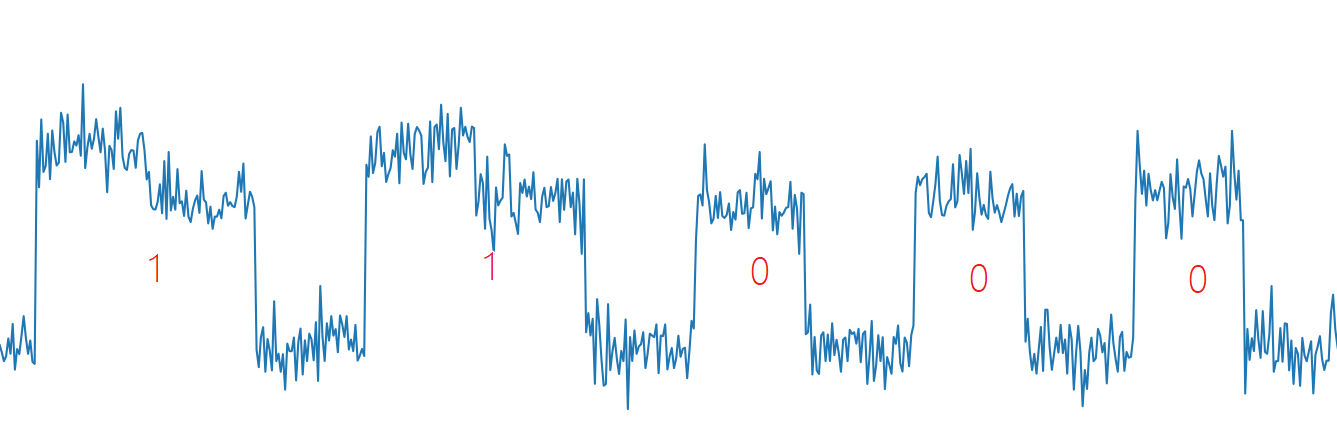
\includegraphics[scale=0.3]{figures/rsa_squaremult.png}
        \label{fig:rsa_squaremult}
    \end{figure}
    As shown in the figure above, by looking at the power consumption we can clearly distinguish whether the exponent
    bit is 1 or 0, and thus we can infer the value of the secret exponent.
\end{example}

\subsubsection{Measurements and attacks}
    When it comes to actually measuring the power consumption of a device we have two main approaches:
    \begin{itemize}
        \item Measure the voltage across a \emph{shunt resistor}: a resistor with a fixed value is placed between the power source
        and the device
        \item Measure the emitted electromagnetic radiation: the current flowing through the device induces magnetic field in the wires, that
        we can pick up with a near-field probe
    \end{itemize}
    Both methods have their pros and cons: the first one is more accurate, but requires to phisically install the shunt resistor on the device;
    the second one is non-intrusive, but the measurements are tipically noisy due to external interferences.

    Regardless of the source of a power trace, there are several possibilities to carry out an attack~\cite{DBLP:journals/cryptography/RandolphD20}, such as:
    \begin{itemize}
        \item Simple Power Analysis: observe the power consumption over a single trace
        \item Differential Power Analysis~\cite{DBLP:conf/crypto/KocherJJ99}: analyze multiple executions over the same algorithm with different inputs to detect small input-dependent differences
        \item Template attacks~\cite{DBLP:conf/ches/ChariRR02}: collect a large number of traces and use them to build a \emph{template} of the power consumption of the device to detect
        when the device is performing a specific operation 
    \end{itemize}

\subsection{Countermeasures}
    The existence of a side-channel does not necessarily mean that an attack is possible: in fact, there are a number of countermeasures
    that can mitigate the risk of a successful attack.

    Regarding timing attacks, the most common countermeasure is to use \emph{constant-time} algorithms, that take the same amount of time to
    execute regardless of the input; this can be achieved, for example, by replacing branching statements that depend on the inputs.

    A very effective way to avoid leakage, especially with respect to power attacks, is to randomize the inputs of the algorithm without
    affecting the output. To do so, we can \emph{mask} the inputs: the basic principle of masking~\cite{DBLP:conf/eurocrypt/ProuffR13} is to split every sensitive value $x$ 
    into $d+1$ \textit{shares}, in such a way that the following relation holds:
    \begin{equation}
        x = x_0 \odot x_1 \odot \cdots \odot x_d
    \end{equation}
    The shares $x_1, \cdots, x_d$ are called \textit{masks} and are randomly sampled, while the secret $x_0$ is processed in 
    such a way that the relation above holds. The goal of masking is to make the sensitive value indistinguishable from
    a random value, so that the observation of a side channel does not reveal any sensitive information, but only random noise.
    There is no particular constraint on the choice of the operation $\odot$ as long as it preserves the relation above;
    in practice, the most common choice is to use the XOR operation, as it is very fast and easy to implement: such a masking
    scheme (e.g.~\cite{DBLP:conf/crypto/IshaiSW03}) is often referred to as \emph{boolean} masking.
    As proven in~\cite{DBLP:conf/crypto/ChariJRR99}, a masking scheme with $d$ shares is a sound counermeasure against a side-channel attack 
    of $d$-th order, where an attacker can have up to $d$ \emph{probes} on the target system; this means that a $d+1$-th order
    attack could be possible, but such attacks become impractical as $d$ increases.



\section{Hamming Quasi-Cyclic}
Hamming Quasi-Cyclic~\cite{melchor2018hamming} is a fourth round candidate in the NIST Post-Quantum cryptography standardization process.
HQC is a code-based cryptosystem, that includes comprises both a public-key encryption (\textsf{HQC.PKE}) and a
key encapsulation mechanism (\textsf{HQC.KEM}).\\
In this section we will describe the inner workings of HQC and show its theoretical security; moreover,
we will give an overview of the currently known attacks against HQC and their practical impact.

\subsection{Encryption scheme}\label{sec:encryption}
We can think of a generic encryption scheme as a tuple of four polynomial time algorithms:
\begin{itemize}
    \item \textsf{Setup}$(1^\lambda)$: generates the global parameters \textsf{param} based on the security parameter $\lambda$.
    \item \textsf{Keygen(param)}: generates a public key \textsf{pk} and a secret key \textsf{sk} based on the global parameters \textsf{param}.
    \item \textsf{Encrypt(pk, \textbf{m}, $\theta$)}: outputs the ciphertext \textbf{c} for the message \textbf{m} with the randomness $\theta$ under the public key \textsf{pk}.
    \item \textsf{Decrypt(sk, \textbf{c})}: outputs the message \textbf{m} for the ciphertext \textbf{c} (or $\bot$ if the ciphertext is invalid).
\end{itemize}

TODO: add security proof?

\subsection{Public Key Encryption}\label{sec:pke}
HQC uses two different codes:
\begin{itemize}
    \item A publicly available decodable code $\mathcal{C} = [n, k]$ generated by $\mathbf{G} \in \mathds{F}_2^{k \times n}$  with an efficient decoding algorithm 
    $\mathcal{C}.\textsf{Decode}()$ which can correct up to $\delta$ errors.
    \item A random double-circulant $[2n,n]$ code with parity-check matrix $\mathbf{H} = (\mathbf{I_n, circ(h)})$. 
\end{itemize}

The \textsf{HQC.PKE} defines the four algorithms of an encryption scheme as follows:
\begin{itemize}
    \item \textsf{Setup}$(1^\lambda)$: generates the set of parameters \textsf{param} = $(n, k, \delta, \omega, \omega_r, \omega_e)$
    \item \textsf{Keygen(param)}: samples $\mathbf{h} \xleftarrow{\mathdollar} \mathcal{R}$ and 
    $(\mathbf{x}, \mathbf{y}) \xleftarrow{\mathdollar} \mathcal{R} \times \mathcal{R}$ such that $\texttt{wt}(\mathbf{x}) = \texttt{wt}(\mathbf{y}) = \omega$;
    the keypair is defined as \textsf{sk} = $(\mathbf{x}, \mathbf{y})$ and \textsf{pk} = $(\mathbf{h}, \mathbf{s} = \mathbf{x} + \mathbf{h\cdot y})$.
    \item \textsf{Encrypt(pk, \textbf{m}, $\theta$)}: samples $\mathbf{e} \xleftarrow{\mathdollar} \mathcal{R}$, $(\mathbf{r_1}, \mathbf{r_2}) \xleftarrow{\mathdollar} \mathcal{R} \times \mathcal{R}$ such that
     $\texttt{wt}(\mathbf{e}) = \omega_e$ and $\texttt{wt}(\mathbf{r_1}) = \texttt{wt}(\mathbf{r_2}) = \omega_e$;  the ciphertext is defined as the pair
     $(\mathbf{u}, \mathbf{v})$, where $\mathbf{u} = \mathbf{r_1} + \mathbf{h}\cdot\mathbf{r_2}$ and $\mathbf{v} = \mathbf{mG} + \mathbf{s\cdot r_2} + \mathbf{e}$.
    \item \textsf{Decrypt(sk, \textbf{c})}: outputs $\mathcal{C}.\textsf{Decode}(\mathbf{v} - \mathbf{u\cdot y})$.
\end{itemize}

The idea at the core of \textsf{HQC.PKE} is to encode the message ($\mathbf{mG}$) and then add random errors that can be removed only by knowing the secret key.\\

TODO: add security proof?

\subsection{Key Encapsulation Mechanism}\label{sec:kem}
In practice, public key encryption is not used to encrypt large amounts of data because of its high exectution time compared to symmetric encryption.
For this reason, we use public key encryption to exchange a shared secret key, which is then used to encrypt the actual data: the practice
of using a public key encryption scheme to exchange a shared secret key is referred to as key encapsulation mechanism (KEM).\\
The Fujisaki-Okamoto transformation~\cite{fujisaki2013secure} is a technique that allows to transform a \textit{weak} IND-CPA encryption scheme
into a \textit{stronger} IND-CCA2 key encapsulation mechanism.

Let $\mathcal{E}$ an instance of \textsf{HQC.PKE} and $\mathcal{G, H}$ and $\mathcal{K}$ hash functions. The \textsf{HQC.KEM} scheme is defined as follows:
\begin{itemize}
    \item \textsf{Setup}$(1^\lambda)$: generates the set of parameters as in \textsf{HQC.PKE.Setup}, where $k$ will be the key size.
    \item \textsf{Keygen(param)}: generates a keypair as in \textsf{HQC.PKE.Keygen}.
    \item \textsf{Encapsulate(pk)}: sample $\mathbf{m} \xleftarrow{\mathdollar} \mathds{F}_2^k$ to derive the randomness $\theta = \mathcal{G}(\mathbf{m})$.
    Generate the ciphertext as $\mathbf{c} = (\mathbf{u, v}) \leftarrow \mathcal{E}.\textsf{Encrypt}(\textsf{pk}, \mathbf{m}, \theta)$ and derive the symmetric key
    as $K \leftarrow \mathcal{K}(\mathbf{m, c})$; send $(\mathbf{c, d} = \mathcal{H}(\mathbf{m})).$
    \item \textsf{Decapsulate}(\textsf{sk}, $\mathbf{c, d}$): decrypt the ciphertext as $\mathbf{m^\prime} = \mathcal{E}.\textsf{Decrypt}(\textsf{sk}, \mathbf{c})$, 
    compute $\theta^\prime = \mathcal{G}(\mathbf{m}^\prime)$ and re-encrypt to get $\mathbf{c^\prime} \leftarrow \mathcal{E}.\textsf{Encrypt}(\textsf{pk}, \mathbf{m^\prime}, \theta)$.
    If $\mathbf{c \neq c^\prime}$ or $\mathbf{d} \neq \mathcal{H}(\mathbf{m^\prime})$ return $\bot$, otherwise derive the shared key $\mathcal{K}(\mathbf{m^\prime, c^\prime})$.
\end{itemize}

TODO: what happens if we do not check $\mathbf{d} == \mathcal{H}(\mathbf{m^\prime})$?

\subsection{Parameters}
HQC has three different parameters sets, for category 1, 3 and 5 respectively. We will refer to the implementations
	of these sets as \texttt{hqc-128}, \texttt{hqc-192} and \texttt{hqc-256}.

	Starting from Round 3, the public code with generator matrix $\mathbf{G}$ is instantiated with a concatenated code, using
	Reed-Solomon and Reed-Muller codes as outer and inner codes, with $n_1$ and $n_2$ lenght of the respective codes; the 
	length of the message is $n$, which is the smallest prime greater than $n_1n_2$ such that $ord_n(2) = n-1$.
	The random code with parity-check matrix $\mathbf{H}$ is instantiated by randomly sampling the vector $\mathbf{h}$
	from $\mathds{F}_2^n$.
	The parameters for the three sets are chosen to bound the decryption failure rate (DFR), and are summarized in Table~\ref{tab:parameters}.
	\begin{table}[ht]\small
		\centering
		\caption{Parameters of HQC}
		% as wide as the page
		\begin{tabularx}{\textwidth}{X|X|X|X|X|X|X}
			Instance & $n_1$ & $n_2$ & $n$ & $\omega$ & $\omega_r = \omega_e$ & $DFR$ \\
			\hline
			\texttt{hqc-128} & 46 & 384 & 17'669 & 66 & 75 & $<2^{-128}$ \\
			\hline
			\texttt{hqc-192} & 56 & 640 & 35'851 & 100 & 114 & $<2^{-192}$ \\
			\hline
			\texttt{hqc-256} & 90 & 640 & 57'637 & 131 & 149 & $<2^{-256}$ \\
		\end{tabularx}
        \label{tab:parameters}
	\end{table}

	\subsection{Memory consumption\\}\label{subsec:memory}
		From this point we assume that $n$ is a prime number with $ord_n(2) = n-1$, as per the parameters of HQC. We recall that 
		$\mathcal{R}$ is the ring of polynomials $\mathds{F}_2[X]/\langle X^n+1\rangle$ and denote with $\mathcal{R}_\omega$ the polynomials
		in $\mathcal{R}$ with $\omega$ non-zero coefficients.
		
		The polynomials $v \in \mathcal{R}$ can be represented in two possible forms:
		\begin{itemize}
			\item sparse, as a vector of size $\omega$ coefficients, $\omega = \texttt{wt}(v)$, where each entry corresponds to the degree of a non-zero coefficient.
			\item dense, as a vector of size $\lceil \frac{n}{\texttt{ws}} \rceil$, where \texttt{ws} is the word size of the target architecture.
		\end{itemize}
		With the aforementioned parameters, the objects on which HQC operates require the amounts of memory summarized in Table~\ref{tab:memory}.
		\begin{table}[ht]\small
			\centering
			\caption{Memory consumption (in bytes)}
			\label{tab:memory}
			% as wide as the page
			\begin{tabular}{c|c|c|c|c|c|c|c}
				Instance & Message & Secret Key & Public Key & Shared Secret & Ciphertext & Dense Poly & Sparse Poly \\
				\hline 
				\texttt{hqc-128} & 16 & 2289 & 2249 & 64 & 4481 & 2209 & 300\\
				\hline
				\texttt{hqc-192} & 24 & 4562 & 4522 & 64 & 9026 & 4482 & 456\\
				\hline
				\texttt{hqc-256} & 32 & 7285 & 7245 & 64 & 14469 & 7205 & 596\\
			\end{tabular}
		\end{table}

		Note that the secret key size refers to the memory required to store a $\textit{processable}$ version of if; the
		secret key can also be stored as a 40B seed, which is then used to generate the actual key material.



\chapter{Implementation}
At the time of writing there are no publicly available implementations of HQC specifically targeting microcontrollers.
In this section we describe our implementation of HQC targeting ARM Cortex-M4 microcontrollers, showing the implementative
details for various multiplication algorithms; moreover, we show the first fully masked implementation of HQC, as a countermeasure
against power side-channel attacks.

\section{Polynomial multiplication}
From a computational standpoint, the most expensive operations in HQC are by far the polynomial multiplications: for this reason,
in order to achieve good performance, it is crucial to pick the best multiplication algorithm for the target architecture.

    The polynomials $v \in \mathcal{R}$ can be represented in two possible forms:
    \begin{itemize}
        \item sparse, as a vector of size $\omega$ coefficients, $\omega = \texttt{wt}(v)$, where each entry corresponds to the degree of a non-zero coefficient.
        \item dense, as a vector of size $\lceil \frac{n}{\texttt{ws}} \rceil$, where \texttt{ws} is the word size of the target architecture.
    \end{itemize}
    With the aforementioned parameters, the objects on which HQC operates require the amounts of memory summarized in Table~\ref{tab:memory}.
    \begin{table}[ht]\small
        \centering
        \caption{Memory consumption (in bytes)}
        % as wide as the page
        \begin{tabular}{c|c|c|c|c|c|c}
            Instance & Message & Secret Key & Public Key  & Ciphertext & Dense Poly & Sparse Poly \\
            \hline 
            \texttt{hqc-128} & 16 & 2289 & 2249 & 4481 & 2209 & 300\\
            \hline
            \texttt{hqc-192} & 24 & 4562 & 4522 & 9026 & 4482 & 456\\
            \hline
            \texttt{hqc-256} & 32 & 7285 & 7245 & 14469 & 7205 & 596\\
        \end{tabular}
        \label{tab:memory}
    \end{table}

Note that the secret key size refers to the memory required to store a $\textit{processable}$ version of if; the
secret key can also be stored as a 40B seed, which is then used to generate the actual key material.

Due to its large memory footprint and the limited resources of the target platform, we will consider only the \texttt{hqc-128} instance.


	% descrivere la moltiplicazione shift & add semplice
	\subsection{Shift and Add}\label{subsec:shift_add}
		In the third round reference implementation of HQC, the polynomial multiplication is implemented using a variant of the schoolbook
		\textit{shift and add} method, recalling that the multiplication in $\mathcal{R}$ of a polynomial by a monomial of degree $i$ 
		can be implemented as a circular shift to the left (\clshift) 	of $i$ positions. Given $a(x)$ in sparse form and $b(x)$ in dense form, the algorithms multiplies $b(x)$ by $x^w$, 
		for all $w$s, where $w$ is a non-zero coefficient of $a(x)$, and then adds the results together:

		\begin{algorithm2e}[H]
			\caption{Sparse polynomial multiplication}
			\KwIn{$a(x) \in \mathcal{R}_\omega$ in sparse form, $b(x) \in \mathcal{R}$ in dense form}
			\KwOut{$c(x) = a(x) \cdot b(x) \in \mathcal{R}$ in dense form}
			\For{$i \gets 0$ \KwTo \texttt{ts}}{
				$\texttt{table}[i] \gets b(x) \clshift i$\;
			}
			\For{$i \gets 0$ \KwTo $\texttt{wt}(a(x))$}{
				$w \gets a(x)[i]$\;
				$\texttt{dec} \gets w \mod \texttt{ts}$\;
				$\texttt{s} \gets \lfloor \frac{w}{\texttt{ts}} \rfloor$\;
				$\texttt{tmp} \gets x^\texttt{s}\cdot x^\texttt{ts}$\;
				$c(x) \gets c(x) + \texttt{table}[\texttt{dec}] \cdot \texttt{tmp}$\;
			}
			\KwRet $c(x) \mod (x^n+1)$\;
		\end{algorithm2e}
		The idea of this variant is to precompute the first \texttt{ts} shifts of $b(x)$ and store them in a table, where \texttt{ts} is set to 16;
		this allows to slightly improve the performance of the algorithm and to shuffle the memory accesses to \texttt{table}.\\
		Since $a$ is very sparse, this approach is extremely fast; however, the high speed achieved is counterbalanced by the
		non-constant time execution of the algorithm, which is a major drawback for the security of the implementation. 

	% descrivere la versione a tempo costante della mul shift & add 
	\subsection{Constant-time shift and add}\label{subsec:const_shift_add}
		Due to the high sparsity of one of the operands, we would like to exploit the fact that the algorithm is very fast to implement a constant-time version of it;
		such an algorithm is implemented in LEDAcrypt~\cite{DBLP:conf/cbc/BaldiBCPS19} and is based on \textit{shifts with conditional commitment}.\\

		\begin{algorithm2e}[H]
			\caption{Constant-time monomial multiplication}
			\KwIn{$a$ exponent of a monomial $x^a \in \mathds{Z}_2[x]$ with $0 \leqslant a < n$, \newline
					$b(x) \in \mathcal{R}$ in dense form}
			\KwOut{$c(x) = x^a \cdot b(x) \in \mathcal{R}$ in dense form}
			\KwData{$m = \lceil \log_2(a) \rceil$ number of bits needed to encode $a$ in binary, \newline
					\textit{i.e.} $a = (\beta_{m-1}, \cdots, \beta_0)_{\texttt{bin}}$}

			$c(x) \gets b(x) \clshift (a \mod \texttt{ws})$\;
			\For{$i \gets \log_2(\texttt{ws})$ \KwTo $(m-1)$} {
				$\texttt{tmp} \gets b(x) \clshift i$\;
				$c(x) \gets c(x) + \texttt{tmp}$\;
				$\texttt{cond} \gets (\beta_{i} == 1)$\;
				$\texttt{mask} \gets 0 - (\texttt{WORD})(\texttt{cond})$\;
				$c(x) \gets c(x) + ((c(x) \wedge \texttt{mask}) \vee (\texttt{tmp}(x) \wedge \texttt{mask}))$\;
			}
			\KwRet $c(x)$\;
		\end{algorithm2e}
		With this algorith we compute the $i$-th shift of $b(x)$ regardless of the value of $\beta_i$, but we sum it to the result only if
		$\beta_i = 1$ (the mask at line 6 contains either all zeros or all ones, '$\vee$' and '$\wedge$' correspond to the bitwise OR and AND respectively).
	% descrivere la moltiplicazione con trasformate

    \subsection{Frobenius Additive FFT}\label{subsec:fafft}
        The implementation of the Frobenius Additive FFT is based on the work of Chen \textit{et.al.}~\cite{DBLP:journals/tches/ChenCK21}; for the sake of clarity, 
        we highlight the core ideas of this implementation.
        
        As shown in Algorithm~\ref{alg:fafft}, the FAFFT multiplication is composed of four components (with the relative inverses): basis conversion, encoding, butterflies and
        pointwise multiplication.
        Our implementation targets a 32-bit platform, hence we pick $m=32$ for the ease of representation of the operands in memory; 
        recalling Equation~\ref{eq:frobenius_partition}, the optimal Frobenius partition for our parameters is $\Sigma = v_{27} + W_{11}$. 
        Since the degree of the operands is fixed, it is possible to optimize these algorithms by unrolling the recursive calls and precomputing the necessary tables.

    \subsubsection{Pointwise multiplication}
        To carry out the 2048 pointwise multiplications in $\mathds{F}_{2^{32}}$ the field elements are represented in a bitsliced format,
        where each element is stored in a memory word. Given  $a$ and $b$ elements in $\mathds{F}_{2^{32}}$, we can compute their product
        by splitting them as $a_0 + a_1\cdot x^{16}$ and $b_0 + b_1\cdot x^{16}$, and computing the product using the Karatsuba multiplication
        algorithm in $\mathds{F}_{2^{16}}$.

    \subsubsection{Basis conversion}
        In Algorithm~\ref{alg:basiscvt}, we show how to convert a polynomial from the canonical to the \emph{novelpoly} basis by recursively
        dividing the input by the vanishing polynomials $s_i(x)$. Since the division by the vanishing polynomial (of largest degree possible) always produces only $h_0(x)$ and $h_1(x)$, 
        we can unroll the recursive calls and transform the algorithm in a binary circuit with only \texttt{XOR} operations; moreover, we can remove all the operations on coefficients
        of the input polynomial that we know are zero.

        \begin{example}[Monomial to novelpoly basis conversion]
            Each step splits the input into quotient and remainder, so we can represent the whole algorithm as a tree, where a node's left child is the remainder and the right child is the quotient:
            by doing so, at the last step of the recursion we can read the leaves, from left to right, as the coefficients $g_0, g_1, \cdots$ of the polynomial in the novelpoly basis.

            Let us take $f(x) = x^6$ in monomial basis and apply the basis conversion algorithm to it. The greatest $i$ such that $2^{2^i} \leqslant \deg(f(x))$ is $i=2$, so at the various
            levels of the tree we will divide the inputs by $s_2(x)=x^4+x$ and $s_1(x)=x^2+x$:
            \begin{figure}[H]
                \caption{Expansion of the basis conversion algorithm for $f(x) = x^6$}
                \begin{center}
                    \begin{forest}
                        [$x^6$[$x^3$[0[0][0]][$x+1$[1][1]]][$x^2$[$x$[0][1]][1[1][0]]]]
                    \end{forest}
                \end{center}
                \label{fig:tree}
            \end{figure}
            hence the representation of $x^6$ in novelpoly basis is $X_2(x) + X_3(x) + X_5(x) + X_6(x)$.

            If we repeat the same procedure with all the required monomials (of degree less than 8 for this case) we can obtain the following circuit that maps coefficients of the 
            canonical basis $f_i$ to coefficients of the novelpoly basis $g_i$, where the dashed line marks the separation between the first two levels of the tree after the root:

            \begin{figure}[H]
    \caption{Basis conversion, $n < 8$}
    \begin{center}
        \begin{tikzpicture}[scale=0.5]
            \node (f0) at (0,7) {$f_0$};
            \node (f1) at (0,6) {$f_1$};
            \node (f2) at (0,5) {$f_2$};
            \node (f3) at (0,4) {$f_3$};
            \node (f4) at (0,3) {$f_4$};
            \node (f5) at (0,2) {$f_5$};
            \node (f6) at (0,1) {$f_6$};
            \node (f7) at (0,0) {$f_7$};
            \node (g0) at (20,7) {$g_0$};
            \node (g1) at (20,6) {$g_1$};
            \node (g2) at (20,5) {$g_2$};
            \node (g3) at (20,4) {$g_3$};
            \node (g4) at (20,3) {$g_4$};
            \node (g5) at (20,2) {$g_5$};
            \node (g6) at (20,1) {$g_6$};
            \node (g7) at (20,0) {$g_7$};

            \node (m1) at (3, 1)  {\tiny$\bullet$};
            \node (m2) at (5, 0)  {\tiny$\bullet$};
            \node (m3) at (7, 3)  {\tiny$\bullet$};
            \node (m4) at (9, 2)  {\tiny$\bullet$};
            \node (m5) at (12, 1) {\tiny$\bullet$};
            \node (m6) at (14, 4) {\tiny$\bullet$};
            \node (m7) at (16, 2) {\tiny$\bullet$};
            \node (m8) at (18, 5) {\tiny$\bullet$};

            \node (a1) at (3, 4)  {$\oplus$};
            \node (a2) at (5, 3)  {$\oplus$};
            \node (a3) at (7, 6)  {$\oplus$};
            \node (a4) at (9, 5)  {$\oplus$};
            \node (a5) at (12, 2) {$\oplus$};
            \node (a6) at (14, 5) {$\oplus$};
            \node (a7) at (16, 3) {$\oplus$};
            \node (a8) at (18, 6) {$\oplus$};

            \draw[-stealth] (f0) -- (g0);
            \draw[-stealth] (f1) -- (g1);
            \draw[-stealth] (f2) -- (g2);
            \draw[-stealth] (f3) -- (g3);
            \draw[-stealth] (f4) -- (g4);
            \draw[-stealth] (f5) -- (g5);
            \draw[-stealth] (f6) -- (g6);
            \draw[-stealth] (f7) -- (g7);

            \draw[-stealth, shorten >=-4.5pt] (m1.center) -- (a1);
            \draw[-stealth, shorten >=-4.5pt] (m2.center) -- (a2);
            \draw[-stealth, shorten >=-4.5pt] (m3.center) -- (a3);
            \draw[-stealth, shorten >=-4.5pt] (m4.center) -- (a4);
            \draw[-stealth, shorten >=-4.5pt] (m5.center) -- (a5);
            \draw[-stealth, shorten >=-4.5pt] (m6.center) -- (a6);
            \draw[-stealth, shorten >=-4.5pt] (m7.center) -- (a7);
            \draw[-stealth, shorten >=-4.5pt] (m8.center) -- (a8);

            \draw[dashed, color=red] (10.5, -1) -- (10.5, 8);

            
        \end{tikzpicture}
    \end{center}
    \label{fig:basisconv} 
\end{figure}
        \end{example}

    \subsubsection{Encoding}
        As shown previously, in the encoding step the multiplication in the truncated butterflies have as one of the factors the basis
        vectors $(s_{l+1}(v_{l+m/2}), \cdots, s_{l+l_m}(v_{l+m/2})) = (v_{m/2-1}, \cdots, v_{m/2-l_m})$; for a fixed $m$ these vectors
        are always the same, so we can rewrite this step as a vector-matrix product, summarized in Algorithm~\ref{alg:encoding}.

    \begin{algorithm2e}[H]
        \caption{Encoding, as a vector-matrix product}
        \label{alg:encoding}
        \KwIn{$f(X) = f_0 + f_1X_1 + \cdots + f_{n-1}X_{n-1} \in \mathds{F}_2[x]_{<n}$}
        \KwOut{$g(X) = g_0 + g_1X_1 + \cdots + g_{n^\prime-1}X_{n^\prime-1} \in \mathds{F}_{2^m}[x]_{<n^\prime}$}
        
        \For{$i \leftarrow 0$ \KwTo $n^\prime-1$}{
            $r_i \gets \prod_{j=0}^{l_m-1} (v_{m/2 - j - 1})^{j_i}$
        }
        \For{$i \leftarrow 0$ \KwTo $n^\prime-1$}{
            $g_i \gets \sum_{j=0}^{m-1}f_{j\cdot n^\prime+i}\cdot r_i$
        }
        \KwRet{$g(X) = g_0 + g_1X_1 + \cdots + g_{n^\prime-1}X_{n^\prime-1}$}
    \end{algorithm2e}
        Since the matrix coefficient is fixed the encoding step is a linear map we can generate a binary circuit
        to carry out this step.

    \subsubsection{Butterflies}
        The multiplication step in the $i$-th layer of the butterflies is always of the form $\beta \cdot p_1(s_1(\beta))$, with
        $\beta \in v_{l+m/2-i}+W_{l-i}$, so it is possible to precompute and store the values of $\beta$ in a static table.
        Moreover, by noticing that $\beta = v + w$ with $w \in W_{l-i}$, we can rewrite a generic multiplication $\beta \cdot \gamma$ as
        $\gamma \cdot v + \gamma \cdot w$: the multiplication by $v$ is performed as a linear map in the same fashion as the encoding step,
        while the multiplication by $w$ is performed by carrying out $32/2^{\lceil \log_2(l-i)\rceil}$ multiplications in the subfield of
        size $2^{2^{\lceil \log_2 (l-i) \rceil}}$, as $w$ is an element of such subfield.
        This approach, as shown empirically in~\cite{DBLP:journals/tches/ChenCK21}, takes the least amount of cycles among the possible approaches.
        

\section{Masking}

    Unlike many other cryptosystems, HQC is \textit{linear} in all its operations, making its primitives to be easily masked entirely.
    In the next algorithms we will use the following notation and conventions:
    \begin{itemize}
        \item $d$: the amount of shares
        \item $\ssplit{a} = (a_0,\ldots,a_{d-1})$: additive share splitting of $a$ in $d$ shares over $\mathcal{R}$
        \item $\sample$: uniform sampling from the right hand side of the equation
        \item $(a+\sum_{i=0}^{d-2} \mathtt{rnd}_i)$: masking of $a$ with $d-1$ masks sampled from the same field of $a$
        \item \textsc{Collapse}(a, \ssplit{b}): sum all shares of $b$, in order, to $a$
    \end{itemize}
    To prove the soundness of our masking scheme we show how the share splitting of an input preserves the output
    with respect to the operations performed by the algorithm, namely addition, multiplication and encoding/decoding.
    We will restrict our attention to the case of $d=2$ shares ($\ssplit{a} = (a\oplus x, x)$ with $x$ random mask) with boolean masks,
    as it is the one used in our implementation, but the same reasoning can be applied for an arbitrary number of shares.

    \paragraph{Addition} Let us consider $\ssplit{a} = (a\oplus x, x)$ and $\ssplit{b} = (b\oplus y, y)$;
    the addition of the two share-split numbers is performed by adding the shares of the same index, getting the result
    \begin{equation*}
        \ssplit{a\oplus b} = (a\oplus x \oplus b\oplus y, x \oplus y) = (a\oplus b\oplus x\oplus y, x \oplus y)
    \end{equation*}
    which, once collapsed, gives the expected result $(a \oplus b \oplus x \oplus y) \oplus (x \oplus y) = a \oplus b$.\\
    In the case of an addition between a share-split number and a constant, we can simply add the constant to the first share of the
    share-split number: in this way we are considering the constant as a share-split number with a zero mask, falling back to the previous case.

    \paragraph*{Multiplication} Let us consider $\ssplit{a} = (a\oplus x, x)$ and $b$; in our setting, all the multiplications
    involve a constant and a share-split value. The multiplication between a constant and a share-split number $\ssplit{a}\cdot b$ is performed by multiplying
    every share of $\ssplit{a}$ by $b$, getting the result 
    \begin{equation*}
        \ssplit{a}\cdot b = ((a\oplus x)\cdot b, x\cdot b) = (a\cdot b \oplus x\cdot b, x\cdot b)
    \end{equation*}
    which, once collapsed, gives the result $(a \cdot b \oplus x \cdot b) \oplus (x \cdot b) = a \cdot b$.

    \paragraph*{Encoding/Decoding} Let us consider $\ssplit{a} = (a\oplus x, x)$; the encoding and decoding of a share-split value
    are performed by simply encoding and decoding each share separately:
    \begin{equation*}
        \begin{aligned}
        \textsc{Encode}(\ssplit{a}) &= (\textsc{Encode}(a\oplus x), \textsc{Encode}(x)) = \ssplit{\textsc{Encode}(a)} = \ssplit{b} \\
        \textsc{Decode}(\ssplit{b}) &= (\textsc{Decode}(b\oplus x), \textsc{Decode}(x))
        \end{aligned}
    \end{equation*}
    When we collapse the decoded shares, we get as a result $\textsc{Decode}(b \oplus x) \oplus \textsc{Decode}(x)$; if the code we are using
    is linear, we can further rewrite this result as
    \begin{equation*}
        (\textsc{Decode}(b) \oplus \textsc{Decode}(x)) \oplus \textsc{Decode}(x) = \textsc{Decode}(b) = a
    \end{equation*}
    correctly decoding the masked value.


    \subsection{Keygen}
    The masking of the key generation algorithm is straightforward: after sampling the private key, we mask $y$ and multiply 
    by $h$ to obtain the share-split version of $s$, which is then collapsed to obtain the public key.
    
    \begin{algorithm2e}[H]
        \caption{Keygen, masked version}
        \KwIn{none}
        \KwOut{$\kpub \in \mathcal{R}\times \mathcal{R}; \kpri \in \mathcal{R} \times \mathcal{R}$}
        $h \sample \mathcal{R}$\;
        $(x,y) \sample \mathcal{R}_\omega \times \mathcal{R}_\omega$\;
        $\ssplit{y} \gets (y+\sum_{i=0}^{d-2} \mathtt{rnd}_i)$\;
        $\ssplit{s} \gets h \ssplit{y}$\;
        $\ssplit{s} \gets x + \ssplit{s}$\tcp*{sum $x$ only to the first share}
        \KwRet $\kpri=(x,y)$, $\kpub = (h,\textsc{Collapse}(\ssplit{s}))$\;
        \end{algorithm2e}

    \subsection{Encrypt}
    In the encryption it is important to protect, other than the message $m$ and the public key $s$, also the random polynomials
    $e,r_1$ and $r_2$, as their leakage would allow an attacker to remove the \textit{excess} errors and decode $m$ from the ciphertext.
    
    \begin{algorithm2e}[H]
        \caption{Encrypt($\kpub$, $m$), masked version}
        \KwData{$\mathbf{G}$: a $\mathds{F}_2^{k \times n}$ matrix generating an efficiently correctable code}
        \KwIn{$\kpub$, $m\in \{0,1\}^k$}
        \KwOut{$c = (u, v) \in \mathcal{R} \times \mathcal{R}$}
        $e \sample \mathcal{R}_{\omega_e}$\;
        $(r_1,r_2) \sample \mathcal{R}_{\omega_r} \times \mathcal{R}_{\omega_r}$\;
        $\ssplit{r_1} \gets (r_1+\sum_{i=0}^{d-2} \mathtt{rnd}_i)$\;
        $\ssplit{r_2} \gets (r_2+\sum_{i=0}^{d-2} \mathtt{rnd}_i)$\;
        $\ssplit{u} \gets \ssplit{r_1} + h\ssplit{r_2}$\;
        $\ssplit{m} \gets (m+\sum_{i=0}^{d-2} \mathtt{rnd}_i) $\;
        $\ssplit{v} \gets \ssplit{m}\mathbf{G} + s \ssplit{r_2} + e $\;
        \KwRet $(\textsc{Collapse}(\ssplit{u}),\textsc{Collapse}(\ssplit{v}))$\;
    \end{algorithm2e}
    When calculating \ssplit{v} it is important to perform the operations reported at line 7 from left to right, to avoid leaking
    information about $e$; in alternative, we can also mask $e$ and then sum it to \ssplit{v}.


    \subsection{Decrypt}
    In the decryption we exploit the linearity of the correctable code: after masking $y$ and multiplying by $u$, we 
    generate a random codeword $\ssplit{\bar{m}}$ and encode it into \ssplit{\bar{c}} to protect $v-uy$ during the decoding.
    After the decoding we can collapse $\ssplit{\bar{m}}$ and the decoded message: since the code is linear, the final result
    is the original message, as if we had performed the decoding on $v-uy$ directly.
    \begin{algorithm2e}
        \caption{Decrypt($\kpri$, $c$), masked version}
        \KwData{$\mathbf{G}$: a $\mathds{F}_2^{k \times n}$ matrix generating an efficiently correctable code}
        \KwIn{$\kpri=(x,y) \in \mathcal{R}_\omega \times \mathcal{R}_\omega$, $c = (u,v) \in \mathcal{R} \times \mathcal{R}$}
        \KwOut{$m\in \{0,1\}^k$}
        $\ssplit{y} \gets (y+\sum_{i=0}^{n-2} \mathtt{rnd}_i)$\;
        $\ssplit{uy} \gets u \ssplit{y}$\;
        $\ssplit{\bar{m}} \sample (\{0,1\}^k)^d$\;
        $\ssplit{\bar{c}} \gets \ssplit{\bar{m}}\mathbf{G}$\; 
        $a \gets \text{\sc Collapse}(v ,\ssplit{\bar{c}})$\;
        $m \gets \text{\sc Decode}(\text{\sc Collapse}(a,\ssplit{uy}))$\;
        \KwRet $\text{\sc Collapse}(m ,\ssplit{\bar{m}})$\;
    \end{algorithm2e}

\chapter{Empirical Evaluations}
We chose the STM32L476RG Nucleo board as our benchmarking platform, featuring 96KB of RAM, 1MB of Flash memory,
a 32-bit ARM Cortex M4 which can be clocked up to 80MHz and a true random number generator.
Due to its large memory footprint and the limited amount of memory available on our target platform,
we take into consideration only the \texttt{hqc-128} instance.

We use \texttt{libopencm3} (1.0.0) as firmware library and compile the project with\newline \texttt{gcc-arm-none-eabi} (7.2.1)
using the \texttt{-O3} optimization flag. The board is clocked at a range of frequencies between 16 and 80 MHz, in order to
evaluate the impact of the memory wait states; the frequencies and corresponding amounts of wait cycles are reported in
the table below:
\begin{table}[ht]
    \centering
    \label{tab:waitstates}
    \begin{tabular}{|c|c|c|c|c|c|}
        \hline
        Frequency (MHz) & 16 & 32 & 48 & 64 & 80 \\
        \hline 
        Wait States & 0 & 1 & 2 & 3 & 4  \\
        \hline    
    \end{tabular}
\end{table}

\subsection{Execution time}
\pgfplotstableread[col sep=comma]{  % enc
    Label, Reference (R3), sparsemul (R3), Reference (R4), sparsemul (R4), FAFFT (R4)
    0,      2726,          18920,           136262,         18965,          8834
    1,      2748,          18937,           138227,         18991,          10107
    2,      2799,          18986,           142093,         19049,          11595
    3,      2886,          19064,           147971,         19154,          13189
    4,      3035,          19196,           155762,         19324,          14856
}\armEncTiming % enc

\pgfplotstableread[col sep=comma]{  % dec
    Label,               Reference (R3), sparsemul (R3), Reference (R4), sparsemul (R3), FAFFT (R4)
    0,                 1942,           9010,           68750,          8915,           5043
    1,                 1950,           9018,           69733,          8926,           5677
    2,                 1965,           9027,           71657,          8941,           6409
    3,                 1989,           9045,           74568,          8958,           7176
    4,                 2024,           9071,           78415,          8998,           7958
}\armDecTiming

\pgfplotstableread[col sep=comma]{  % encaps
    Label,           Reference (R3), sparsemul (R3), Reference (R4), sparsemul (R4), FAFFT (R4)
    0,                 3913,           20105,          137873,         20571,          10441
    1,                 3958,           20148,          139835,         20643,          11763
    2,                 4079,           20261,          143631,         20783,          13333
    3,                 4289,           20461,          149685,         21051,          15087
    4,                 4626,           20787,          157722,         21473,          16994
}\armEncapsTiming

\pgfplotstableread[col sep=comma]{  % decaps
    Label,               Reference (R3), sparsemul (R3), Reference (R4), sparsemul (R4), FAFFT (R4)
    0,                 5923,           29182,          206691,         29557,          15546
    1,                 5974,           29230,          209618,         29634,          17504
    2,                 6110,           29361,          215263,         29795,          19804
    3,                 6341,           29578,          224238,         30084,          22326
    4,                 6724,           29926,          236118,         30540,          25015
}\armDecapsTiming

\pgfplotstableread[col sep=comma]{  % mult
    Label,               Reference (R3), sparsemul (R3), Reference (R4), sparsemul (R4), FAFFT (R4)
    0,                 848,            7897,           66777,          7791,           3062
    1,                 848,            7897,           67747,          7791,           3688
    2,                 851,            7897,           69653,          7791,           4404
    3,                 856,            7897,           72537,          7791,           5146
    4,                 862,            7897,           76345,          7791,           5892
}\armMultTiming
  % contains data for the plots

To measure the execution times we use the Data Watchpoint and Trace Cycle Count Register (\texttt{DWT\_CYCCNT}),
a 32-bit register that counts the number of clock cycles elapsed since its last reset with a resolution
of one clock cycle. To avoid overflows, we reset the register after all the measurements of a single round
are completed; to reduce uncertainty, we average the measurements taken over 1000 rounds.
\subsection{Welch's t-test}
To evaluate the existence of an eventual side-channel vulnerability we use the Test Vector Leakage Assessment (TVLA)~\cite{schneider2015leakage},
based on Welch's t-test. The aim of the test is to provide a quantitative measure of how much the means of two
populations differ; the t-test statistic is computed as follows:
\begin{equation}
    t = \frac{\mu_0 - \mu_1}{\sqrt{\frac{s_0^2}{n_0} + \frac{s_1^2}{n_1}}}
\end{equation}  
where $\mu, s^2$ and $n$ are the mean, variance and number of samples of the two populations, respectively.
Small $t$ values give evidence to accept the null hypothesis that the two populations have the same mean; 
usually, for the sake of simplicity, a threshold of $|t| > 4.5$ is defined to reject the null hypothesis with
a confidence level of $99,999\%$.\\
In our case, we take the populations to be the execution times of an algorithm, where in the first we draw
new inputs randomly each time, while in the second we use the same inputs for all the rounds; each population
is composed of 1000 samples.\\

\chapter{Conclusions}
In this thesis we provided the first constant-time implementation of HQC and the
first masked implementation of HQC's public key encryption scheme.

To do so, we evaluated different multiplication methods in terms of both performance and constant-time behavior, 
crowning the Frobenius Additive FFT as the best one on the ARM Cortex-M4 and the Karatsuba algorithm on x86 architectures;
moreover, we implemented a masking scheme for the key generation, encryption and decryption primitives
of HQC's public key encryption scheme.

We provided a comparative analysis of the Round 4 NIST PQC candidates, showing how both our constant-time and masked implementations 
of HQC offer a good trade-off in terms of memory consumption and execution time, making them suitable for the standardization.

As future work, it could be possible to run more accurate tests in order to evaluate the efficacy of our masking scheme against power attacks.
Since our masking scheme targets the PKE only, it could also be possible to extend the masking scheme to 
the SHAKE functions and make the whole KEM secure against power attacks, such as the one proposed in~\cite{DBLP:journals/tches/UenoXTITH22}.


%-------------------------------------------------------------------------
%	BIBLIOGRAPHY\
%-------------------------------------------------------------------------

\addtocontents{toc}{\vspace{2em}} % Add a gap in the Contents, for aesthetics
\bibliography{refs.bib} % The references information are stored in the file named "Thesis_bibliography.bib"

%-------------------------------------------------------------------------
%	APPENDICES
%-------------------------------------------------------------------------

\cleardoublepage
\addtocontents{toc}{\vspace{2em}} % Add a gap in the Contents, for aesthetics
\appendix
\chapter{Appendix A}
Appendix

% LIST OF FIGURES
\listoffigures

% LIST OF TABLES
\listoftables

% ACKNOWLEDGEMENTS
\chapter*{Acknowledgements}
Here you might want to acknowledge someone.

\cleardoublepage

\end{document}
